
\chapter{\textit{Pūrva-pakṣa} of Sheldon Pollock's Use of Chronology}\index{Chronology}\label{chapter1}

\Authorline{-- Manogna Sastry and}

\Authorline{Megh Kalyanasundaram}\footnote{pp. 17-66. In: Kannan, K. S. and Meera H. R. (Ed.s) (2020). \textit{Chronology and Causation: Negating Neo-Orientalism.} Chennai: Infinity Foundation India.}

\lhead[{\small\thepage}\quad\small Manogna Sastry and Megh Kalyanasundaram]{}

\begin{flushright}
\textit{(manognashastry@gmail.com}\\\textit{kalyanasundaram.megh@gmail.com)}
\end{flushright}


\section*{Abstract}

Prof. Sheldon Pollock’s\index{Pollock, Sheldon} body of work shows his penchant for a few pet topics: his positioning Buddhism\index{Buddhism} as the silver bullet that saved the ‘Indian’ from Vedic and Brahmanic oppression and his strenuous case to uncover tenuous parallels between Greek classics and Indian epics, effectively taking away the Indian claim to deeply native and formative elements of her culture. The dismissal of centuries of indigenous oral traditions, a strategic emphasis on deliberately limited aspects of the essence and historicity of  \textit{kāvya}\index{kavya@\textit{kāvya}} in evaluating its contributive value, his theorisation of a perceived tension between Sanskrit and the regional languages as well as his position that the field of Sanskrit has not had a history of examining its own literary change, among other similar fantastic claims, constitute some of his key arguments. When different works from his scholarship are considered together, not only do logical and chronological inconsistencies become evident, but also the near-absence of a detailed chronology, which in his own words is ‘central to comparative intellectual-historical practice.’ Ergo, we present a detailed consolidation of his dispersed chronological data into a framework and proceed to address questions such as—“Does tradition disagree with some of the dates he assigns? Which ones and with what evidence or logic do traditional scholars disagree with Pollock?”—with a particular focus on the epoch around the first of the ``two great moments of transformation in culture and power in premodern India" (Pollock 2006:1) when the supposed ‘momentous rupture’ that led Sanskrit to descend from ‘The World of Gods’ to ‘the World of Men.’ Particular recurrent themes in Pollock’s\index{Pollock, Sheldon} work as well as the larger context he provides for the study and revival (or a case for no revival) of Sanskrit, in context of his chronology\index{Chronology}, are also probed in this paper.




\section*{1. Introduction}

Over the course of its long unbroken history, India has had several encounters with the West, with some that have been mutually enriching while others, challenging and nearly destroying everything she has held as precious and sacred. What could not be destroyed has been left maligned and vilified, with massive ramifications that have changed the very course of her flow several times. Yet, one cannot think of another country, that has faced the sheer number and intensity of assaults that India has, and survived and risen again. When one considers the treasure that every nation brings to the world, India stands tall as one who sought after Infinity, beyond Life and Death, and understood it in all its intensities and hues. She strove to bring that aspiration into everything she realised and built in her world. If she manifested the \textit{veda}-s, the \textit{upaniṣad}-s, and the \textit{śāstra}-s, she also created structures of unimaginable beauty and intellectual precision, in her arts and architecture and literature and sciences, casting her unparalleled keenness of sense to even the smallest of everyday acts. War, statecraft, human psychology — no arena was spared. The space she created, for the \textit{nāstika}\index{nastika@\textit{nāstika}} to exist and thrive and express with as much freedom as the devout \textit{bhakta} is a testament to her vision. This state of being, where all was a simultaneous seeking and expression of the Divine within and without man, has driven one of the oldest civilisations of the world. The master key to the Indian mind is not merely seen in the reflections of his philosophical, intellectual, rational or emotional mind, but, in the spiritual ethos that drives his very being.

However, history has shown how it has been at times a most arduous battle for India to fight and defend. Every encounter she has had with the outsider, especially in the last thousand years, has left her in an increasingly enfeebled state. The very fact that she has survived is a testament to her inner spirit, but, the survival and the price she paid for her political freedom has seen her wealth, in all domains, looted. Analysis, exegesis, interpretation of Indological elements are now carried out primarily by outsiders even as it is the Indian who bears the burden of a history that has been written and shaped and continues to be in various forms, by forces of colonialism. Studies about India now bear three distinctive phases, though work in each of them is evolving concomitantly. Scholarship in pre-colonial, colonial and post-colonial critiques of Indology today finds itself charged with western methods that seek to reckon Indological components through leitmotifs of power and domination. But, scholars from the post-colonial age, while wielding theories and models characteristic of their times, continue to base their constructs on ‘evidence’ and ‘facts’ that were methodically built as a part of creating knowledge about India for the purposes of colonial rule. Thus, while newer and different perspectives on India during its various epochs in her long history continue to be generated, there has been little significance attached to examining the very ‘facts’ that have been taken for an objective given and built further upon.

In spite of the recognition by the domain today, that in creating a picture of India, commissioned by the East India\index{East India Company} Company as it assumed the role of a ruler, several indigenous voices were silenced and never made it to the authoritative, sanctioned canvas, Indologists continue to use these fabricated falsities. And Sheldon Pollock\index{Pollock, Sheldon}, a leading American Indologist studies, is no different in this regard. Pollock expresses mild disdain at several places for ideas from European Orientalism, including dismissing the regard some Oriental Indologists had for India as just Romanticism\index{Romanticism}, but, clearly uses the chronological data built during the period. Even as he professes to be a lover of Sanskrit, his narratives of the language and everything it has represented in India are replete with intellectual \textit{parti pris}. Recurrent major themes in his voluminous scholarship include setting up dichotomies between Hinduism and Buddhism\index{Buddhism}, Sanskrit and the regional languages and often positioning the outsider as someone who saved the language and the society while the native actively used the same as tools of oppression the latter being perhaps the least obvious. Pollock’s hypotheses include incredible ideas that \textit{kāvya}\index{kavya@\textit{kāvya}} was invented around the beginning of CE and its arrival brought down the language from the realm of Gods, thusly presenting a bizarre and incongruous picture of ancient India for the preceding millennia, where one of the greatest civilizations of the world seems to have had little life outside of Vedic chanting and oppressive Brahmanical paraphernalia, which, according to Pollock\index{Pollock, Sheldon}, includes even grammar!

The first five lines of the introduction of Pollock’s magnum-opus\endnote{ Refer Gould (2008).} \textit{The Language of the Gods in the World of Men} should make evident the centrality of Chronology\index{Chronology} to his book’s attempt and therefore, to his theorizations and conclusions:

\begin{myquote}
“This book is an attempt to understand two great moments of transformation in culture and power in premodern India. The first occurred around the beginning of Common Era, when Sanskrit, long a sacred language restricted to religious practice, was reinvented as a code for literary and political expression. …The second moment occurred during the beginning of the second millennium, when local speech forms were newly dignified as literary languages and began to challenge Sanskrit for the work of both poetry and polity, and in the end replaced it.” 

~\hfill (Pollock 2006:01)
\end{myquote}

That Pollock chose to frame the whole “attempt” of his book as “to understand two great moments” naturally necessitates that his methods, theorizations and conclusions are evidently and irrevocably linked to chronology. Consequently, if his assumptions and implications are not chronologically fool-proof, his theorizations and conclusions, at least some if not all, may need to be declared suspect and be revisited for validity, if not completely discredited. The first of the “two great moments” referred to above is in large part, the focus of this paper —the scope has been limited by the authors to the period of BCE — which is an attempt to address some questions including “Does tradition disagree with some of the dates he assigns? Which ones and with what evidence or logic do traditional scholars disagree with SP? Are there other examples in his work that show bias?”\endnote{ \url{https://swadeshiindology.com/si-2/position-papers/}} In addition, we aim to identify internal inconsistencies, if any, in his own chronological data, with the objective of a more comprehensive \textit{pūrva-pakṣa} of his chronology with regard to the first great “moment” and pinpoint which of the theories, particularly those he claims are his (or ascribed exclusively to him in the academia), become questionable.

\bigskip

A survey of Pollock’s works makes evident a stumbling block: the lack of a consolidated, sequentially-arranged view of chronological data,\endnote{ The disproportionate (in relation to the volume of the dates used in his scholarship) and mostly unreferenced data in Appendix B.1 (Pollock\index{Pollock, Sheldon}:2006; 597) is clearly the solitary exception.} necessitating, as first step a clear and sufficiently comprehensive reconstruction of his Chronology\index{Chronology}, in order to identify his chronological assumptions, its sources and their validity, and compare them with data across specifically selected influential scholars who could be seen as belonging to different points of the spectrum bounded by the qualifications of “Insider and Outsider.”\endnote{ Unless specified otherwise, Outsiders and Insiders used throughout this paper are in the sense seen in Malhotra\index{Malhotra, Rajiv}, Rajiv (2016). \textit{Insiders versus Outsiders: Who speaks for our heritage?} \url{https://battleforsanskrit.com/insiders-versus-outsiders/}} One of the outcomes of the analysis is also to arrive at and propose a checklist of ‘chronological “poison-pills”’\endnote{ Refer Malhotra, Rajiv (2014) \textit{Indra’s Net,} Chapter Conclusion: The ‘Poison Pill’\index{poison pills} for Protection of Hinduism.} that could be used as a tool-kit by anyone in the future, to quickly assess and classify narratives in the insider-outsider spectrum. This spectrum is entirely non-political in nature, even as a scholar in the spectrum can subscribe to narratives which may represent insider accounts on a given chronological milestone while to an outsider narrative on any other.

\bigskip

\section*{2. Sheldon Pollock’s\index{Pollock, Sheldon} Chronology}

\smallskip
\smallskip

While a first reconstruction and clear presentation of some aspects of Pollock’s chronology as part of a \textit{pūrva-pakṣa}\index{purvapaksa@\textit{pūrva-pakṣa}} with a scope much larger than that of this paper is found in \textit{The Battle for Sanskrit} by Rajiv Malhotra\index{Malhotra, Rajiv}, a consolidated study of the chronological data that we could find diffused throughout Pollock’s works leads to Tables 1 and 2:

\newpage

\textbf{Table 1: Sheldon Pollock’s Chronology reconstructed from some of his scholarship}

\begin{longtable}{|l|p{1.9cm}|p{1.9cm}|p{1.6cm}|p{1.2cm}|}
\hline
Sl. No. & \multicolumn{2}{c|}{Epoch} & Referenced (Yes/No) & Source \\
\hline
 & Period/Date & Detail &  &  \\
\hline
1 & 1000 BCE (Beginning of first\break millennium BCE) & Earliest form of Sanskrit appeared in South Asia & No & Pollock 2006:39 \\
\hline
2 & 1000 – 1 BCE (Entire first millennium BCE) & \textit{Vaidika} Sanskrit culture: Prevalence of its liturgical dimension and restriction of its use & No & Pollock 2006:67 \\
\hline
3 & 550 – 330 BCE & Achaemenids\index{Achaemenids} & Yes (elsewhere) & Pollock 2006:597 \\
\hline
4 & 527 BCE & Mahāvīra\index{Mahavira@Mahāvīra} & Ascribed to tradi\break tion without being specific & Pollock 2006:424 \\
\hline
5 & 500 – 400 BCE & Rise of Buddhism\index{Buddhism} & No & Pollock\index{Pollock, Sheldon} 2003:85 \\
\hline
6 & c. 400 BCE & Buddha\index{Buddha, the} & No & Pollock 2006:81 \\
\hline
7 & Mid fourth century BCE & Pāṇini\index{Panini@Pāṇini} & Ascribes to conven\break tion without being specific & Pollock 2006:81 \\
\hline
8 & 400 – 200 BCE & Sanskrit grammatical tradition synthesized around third or fourth century BCE & No & Pollock 2003:62 \\
\hline
9 & 400 – 200 BCE & Pāṇini’s \textit{Aṣṭādhyāyī}\index{Astadhyayi@\textit{Aṣṭādhyāyī}} & No & Pollock 2006:45 \\
\hline
10 & 400 – 200 BCE & \textit{Vinaya piṭaka} (text) & Yes & Pollock 2006:54 \\
\hline
11 & 320 – 150 BCE & Maurya dynasty & No & Pollock 2006:59 \\
\hline
12 & 320 – 150 BCE & Mauryas & No & Pollock 2006:597 \\
\hline
13 & 300 – 200 BCE & Latin firmly rooted in Central Italy & No & Pollock 2006:20 \\
\hline
14 & 300 – 200 BCE & Chi’in Shih Huang-ti dynasty & No & Pollock 2006:535 \\
\hline
15 & 264 – 241 BCE & First Punic War & No & Pollock 2006:264 \\
\hline
16 & Around 260 BCE & Invention of writing itself in India & Ascribed to a ‘new scholarly consensus’ without specifying & Pollock 2006:81 \\
\hline
17 & Middle of third century BCE & Promulgation of edicts during Aśoka’s\index{Asoka@Aśoka}\index{Asokan edicts@Aśokan edicts} chancery & Yes & Pollock\index{Pollock, Sheldon} 2006:59 \\
\hline
18 & Middle of third century BCE & Brahmi syllabary, first South Asian writing system & Yes & Pollock 2006:59 \\
\hline
19 & Mid-third century BCE onwards & Prakrit, the voice of polity & No & Pollock 2006:499 \\
\hline
20 & Mid-third century BCE & Beginning of expression of political will by ruling lineages & Ascribed to Aśokan edicts & Pollock 2006:331 \\
\hline
21 & Mid-third century BCE & Translation of Aśokan\index{Asoka@Aśoka}\index{Asokan edicts@Aśokan edicts} edicts into literary Greek & No & Pollock 2006:265 \\
\hline
22 & Third century BCE & New cultural inputs from the west & No & Pollock 2006:537 \\
\hline
23 & Mid-third century BCE & Outermost historical limit of Vālmīki’s\index{Valmiki@Vālmīki} \textit{kāvya}\index{kavya@\textit{kāvya}} & Not clear & Pollock 2003:87 \\
\hline
24 & Last centuries BCE & No evidence compels belief of existence of \textit{kāvya} before last centuries B.C.E, if that early & Not clear & Pollock 2003:84 \\
\hline
25 & Third century BCE to first century CE & Early epoch of literacy: no remains of non-sacral, this-worldly Sanskrit extant \textit{with the exception of} \textit{Rāmāyaṇa}\index{Ramayana@\textit{Rāmāyaṇa}} & No & Pollock\index{Pollock, Sheldon} 2006:48 \\
\hline
26 & 225 BCE – 250 CE & Sātavāhanas\index{Satavahana@Sātavāhana} & No & Pollock 2006:597 \\
\hline
27 & 225 BCE – 250 CE & Sātavāhanas & Yes & Pollock 2006:61 \\
\hline
28 & Last centuries (most probably third or second) BCE & \textit{Mīmāṁsāsūtra}\index{Mimamsa@Mīmāṁsā} & No & Pollock 2006:40 \\
\hline
29 & d. 204 BCE & Naevius\index{Naevius} – Latin poet from today’s Naples & No & Pollock 2006:264 \\
\hline
30 & Last two centuries BCE & Tamil Brahmi cave inscriptions & Yes & Pollock 2006:290 \\
\hline
31 & About second century BCE & Kātyāyana\index{Katyayana@Kātyāyana} & Not clear & Pollock 2006:385 \\
\hline
32 & Last century or two before the beginning of CE & Development of \textit{kāvya}\index{kavya@\textit{kāvya}} & No & Pollock 2003:85 \\
\hline
33 & Second century BCE & Sinhaḷa literized & No & Pollock\index{Pollock, Sheldon} 2006:386 \\
\hline
34 & d. 169 BCE & Ennius, Latin poet from Calabria & Yes & Pollock 2006:264 \\
\hline
35 & 100 BCE – 400 CE & Śakas\index{Saka@Śaka}\index{Kusanas@Kuṣāṇas} and Kuṣāṇas & No & Pollock 2006:597 \\
\hline
36 & c. 100 BCE – 250 CE & Sātavāhanas\index{Satavahana@Sātavāhana} & No & Pollock 2003:70 \\
\hline
37 & From probably first century BCE & Earliest documents in Sanskrit & No & Pollock 2006:60 \\
\hline
38 & From not much before Common era & Outer limit for Sanskrit \textit{Mahābhārata}\index{Mahabharata@\textit{Mahābhārata}} & No & Pollock 2006:224 \\
\hline
39 & Middle of first century BCE & Arrival of Śakas\index{Saka@Śaka} & Yes & Pollock 2006:70 \\
\hline
40 & End of first century BCE & Disappearance of all Italian languages from inscriptional record save Latin & No & Pollock 2006:271 \\
\hline
41 & About 150 CE & Nasik cave inscription of Gautamī Bālaśrī & No & Pollock 2006:238 \\
\hline
42 & Middle of second century & Patañjali\index{Patanjali@Patañjali} & Yes & Pollock 2003:84 \\
\hline
43 & Mid second century & Invention of Indian astrology by translation of Hellenistic horoscopy into Sanskrit by “Lord of the Greeks” & Yes & Pollock\index{Pollock, Sheldon} 2006:537 \\
\hline
44 & 149-150 CE & Middle of the reign of Rudradāman;\index{Rudradaman@Rudradāman} unprecedented sculpture of Gāndhāra & Yes & Pollock 2006:265 \\
\hline
45 & In second century and onwards & Beginning of usage of Sanskrit for public texts & No & Pollock 2003:84 \\
\hline
46 & 200 – 400 CE & Dating of Vararuci\index{Vararuci} & No & Pollock 2006:101 \\
\hline
47 & Around 225 CE & Ikṣvākus\index{Iksvakus@Ikṣvākus} & Yes & Pollock 2006:116 \\
\hline
48 & 225 – 300 CE & Ikṣvākus & No & Pollock 2006:597 \\
\hline
49 & 250 – 500 CE & Vākāṭakas\index{Vakataka@Vākāṭakas} & No & Pollock 2006:597 \\
\hline
50 & 300 – 600 CE & Kadambas\index{Kadamba} & No & Pollock 2006:597 \\
\hline
51 & 300 – 900 CE & Pallavas\index{Pallavas} & No & Pollock 2006:597 \\
\hline
52 & c. 300 & \textit{Nāṭyaśāstra}\index{Natyasastra@\textit{Nāṭyaśāstra}} & No & Pollock 2016:132 \\
\hline
53 & Early CE & \textit{Stotra} & No & Pollock\index{Pollock, Sheldon} 2016:83 \\
\hline
54 & 320 – 550 CE & Guptas\index{Guptas} & No & Pollock 2006:597 \\
\hline
55 & 400 – 1000 CE & Gaṅgas\index{Gangas@Gaṅgas} & No & Pollock 2006:597 \\
\hline
56 & Fifth century CE & Beginning of literization\index{literization} of Kannada & No & Pollock 2006:26 \\
\hline
57 & 500 – 750 CE & Bādāmi Cāḷukyas\index{Calukyas@Cāḷukyas} & No & Pollock 2006:597 \\
\hline
58 & 5th or 6th century CE & Weakening and breaking of Prakrit as a medium for \textit{kāvya}\index{kavya@\textit{kāvya}} & No & Pollock 2006:101 \\
\hline
59 & 600 – 700 CE & First appearance of literary-theoretical reflection & No & Pollock 2006:13 \\
\hline
60 & 600 – 700 CE & Kumārila\index{Kumarila Bhatta@Kumārila Bhaṭṭa} & No & Pollock 2006:500 \\
\hline
61 & 600 – 1300 CE & Pāṇṭiyas\index{Pantiyas@Pāṇṭiyas} & No & Pollock 2006:597 \\
\hline
62 & 625 – 1075 CE & Veṅgi Cālukyas\index{Calukyas@Cālukyas} & No & Pollock 2006:597 \\
\hline
63 & Mid-7th century CE  & Plays, discovered in Trivandrum in early 1900’s, ascribed to Bhāsa\index{Bhasa@Bhāsa} & Not clear & Pollock 2006:81\break  Pollock 2003:85 \\
\hline
64 & Late-7th century ~700 CE & \textit{Kāvyādarśa}\index{Kavyadarsa@\textit{Kāvyādarśa}} of Daṇḍin\index{Dandin@Daṇḍin} & No & Pollock\index{Pollock, Sheldon} 2006:163 \\
\hline
65 & 725 – 950 CE & Gurjara Pratīhāras\index{Pratiharas@Pratīhāras} & No & Pollock 2006:597 \\
\hline
66 & 750 – 1200 CE & Pālas\index{Palas@Pālas} & No & Pollock 2006:597 \\
\hline
67 & 750 – 975 CE & Rāṣṭrakūṭas\index{Rastrakuta@Rāṣṭrakūṭa} & No & Pollock 2006:597 \\
\hline
68 & 779 CE & \textit{Kuvalayamālā}\index{Kuvalayamala@\textit{Kuvalayamālā}} & Yes & Pollock 2006:96 \\
\hline
69 & 700 – 800 CE & Śaṅkara\index{Sankara@Śaṅkara} & No & Pollock 2006:570 \\
\hline
\end{longtable}

(A continuation of this Table 1 can be found in the Appendix; Table 2 in Appendix is an exclusive chronological tabulation of texts (with their Pollock-assigned English names), reconstructed from Pollock’s book: \textit{A Rasa\index{rasa@\textit{rasa}} Reader: Classical Indian Aesthetics})

%\newpage


\section*{3. Pollock’s Chronology\index{Chronology} – \hfill\break Analysis and Insights}

\subsection*{3.1 Internal Inconsistencies in Pollock’s Data}

In light of the scope of the paper limited to the BCE period, among the 40 BCE points in Table 1, one observes that a conspicuous 24 lack any references. We also observe that some data within Pollock’s own work are inconsistent with each other. From Table 1, at least two such internal inconsistencies can be identified, the first more distinct than the second.

\subsubsection*{3.1.1 Sātavāhana-s}\index{Satavahana@Sātavāhana}

In Pollock (2003), one finds “Staunchly Brahmanical lineages to the south such as the Sātavāhanas (c. 100 B.C.E–250 C.E.) held to the old ways and supported no literary production whatever in Sanskrit,” (Pollock\index{Pollock, Sheldon} 2003:70). But in \textit{The Language of the Gods in the World of Men} we see respectively, “Sātavāhanas 225 b.c.e.–250 c.e.” (Pollock 2006:597) and

\begin{myquote}
“Yet this explanation seems to be refuted by a simple fact, one that is no mere artifact of our data: in the early period of literacy in South Asia, no dynasty, regardless of how \textit{vaidika} it was—and therefore, according to the logic of the religious argument, both willing and able to use Sanskrit—employed that language for its public records. Exemplary here are the cultural practices of the Sātavāhanas. This lineage exercised some form of rule over a wide area of southern India from about 225 b.c.e. to 250 c.e. From the large body of Sātavāhana inscriptional and numismatic evidence available to us now, a very striking kind of cultural politics emerges. This was a lineage of rulers who unequivocally saw themselves inhabiting a Vedic world, as evidenced by both their continual performance of the solemn ceremonies of the Srauta tradition and their explicit self-identification as Brahmanical.” 

~\hfill (Pollock\index{Pollock, Sheldon} 2006:61)
\end{myquote}

Thus, we see a 125-year difference in the start year across his two books and its significance is evident from the importance he himself attaches to this lineage.

\subsubsection*{3.1.2 Vararuci}\index{Vararuci}

In Pollock(2003), one finds

\begin{myquote}
“From among the vast library of early Sanskrit texts, no evidence compels belief in the existence of \textit{kāvya}\index{kavya@\textit{kāvya}} before the last centuries b.c.e, if that early. Our first actual citations of Sanskrit \textit{kāvya} are found in Patañjali’s\index{Patanjali@Patañjali} \textit{Mahābhāṣya}\index{Mahabhasya@\textit{Mahābhāṣya}} (Great commentary) on the grammar of Pāṇini.\index{Panini@Pāṇini} The materials he cites, if astonishingly thin for a work on the Sanskrit language some 1500 printed pages in length, suggest a state of \textit{kāvya} reasonably developed in form and convention 99. The problem is not the date of literary culture in the \textit{Mahābhāṣya}, however meager, but the date of the author, Patañjali. The evidence usually adduced for an early date is ambiguous and meager; the most compelling arguments place him earlier than the middle of the second century of the common era.” 

~\hfill (Pollock 2003:84)
\end{myquote}

If dating Patañjali to c. 150 CE (i.e. ‘middle of the second century of common era’) was itself not distortion enough, footnote 99 holds the key to another: “Patañjali, however, refers to a poet by name only once, mentioned “the poem composed by Vararuci (\textit{vārarucaṁ kāvyam}, on 4.3.101)”” (Pollock 2003:84). For a moment, if one were to admit Pollock’s dating of Patañjali, Vararuci should, according to his own footnote 99, predate his dating of Patañjali, i.e. date to a period before c. 150 CE. In Pollock (2006) though, one finds the following

\begin{myquote}
“A major factor in the process was philology in the wide sense of the term. Both Prakrit and Apabhhramsha came under the standardizing pressure of a growing scholarly apparatus—newly created grammars, dictionaries, metrical handbooks, dramaturgical treatises, and so forth—that thoroughly bears the stamp of Sanskrit. Instructive here is the earliest systematization of Maharashtri Prakrit, the \textit{Prākṛtrasūtra} (or -\textit{prakāśa}, the Rules of Prakrit, or Light on Prakrit), a grammar composed in perhaps third or fourth century by Vararuci (at least in its core form; chapters for the other Prakrits were added at a later date).” 

~\hfill (Pollock 2006:101)
\end{myquote}

From review of the footnote 99 in LCIH and the above statement, one of two inferences is tenable: either Pollock’s data is inconsistent or that he implies the existence of two Vararuci-s; yet both these inferences would implicate Pollock. Explaining away that the two Vararuci-s above as different would not be sufficient, in light of again, Pollock’s own expansions, this time on Kātyāyana\index{Katyayana@Kātyāyana}, as found in \textit{The Language of the Gods in the World of Men}, wherein, in addition to dating Kātyāyana to “about second century b.c.e” (Pollock 2006:385), he not only acknowledges the \textit{Vārttika} of Kātyāyana\index{Katyayana@Kātyāyana} and that it was found in \textit{Mahābhāṣya}\index{Mahabhasya@\textit{Mahābhāṣya}} in vol 1:12 but also places Kātyāyana, like traditionalists, “between the time of Pāṇini\index{Panini@Pāṇini} and Patañjali\index{Patanjali@Patañjali}” (Pollock 2006:47). Yet, his dismissal of the scholarship of eminent insider Krishnamachariar\index{Krishnamachariar, M.} to a footnote\endnote{Refer Pollock (2003:84), Footnote 9.} is only matched by his willful omission or ignorance of the well-known traditional account of Vararuci\index{Vararuci} being the other name of Kātyāyana. Krishnamachariar wrote, in his \textit{History of Classical Sanskrit Literature}:

\begin{myquote}
“Vararuci also called Kātyāyana was the son of Somadatta\index{Somadatta} of Sankjti gotra\index{gotra@\textit{gotra}}. He was born at Kauśāmbi on the Jumnā. He studied along with Pāṇini and Vyādi under the Upavarśa in Pātaliputra and married his daughter Upakośa. He composed the Vārtika on Pāṇini and the ślokas called \textit{Bhrajas Patañjali}. Patañjali in his \textit{Mahabhashya} (1. 23) mentions a poem by him (IV iii). According to the Avanti-Sundarī-Kathāsāra (IV 17) Vararuci was born in the reign of King Mahāpadma, son of King Mahānandi son of Nandivardhana, who ruled of Visālā. According to the Purānas, ruled for 43 years from 1678 to 1635 BC.” 

~\hfill (Krishnamachariar 1937:86) \textit{(Spelling and italics as in the Original)}
\end{myquote}

In light of the above, even without taking into account the dating of Vararuci as per insider accounts such as that proposed by M. Krishnamachariar, does not the difference in Pollock’s\index{Pollock, Sheldon} own date for Vararuci and Kātyāyana, instantiate a clear case of chronological inconsistency, perhaps willful omission of key information and muddled methodology featuring list-and-dismiss tendencies? A Pollock-acknowledged Vararuci between Pāṇini and Patañjali with a traditional dating would seriously affect his theorization of \textit{kāvya},\index{kavya@\textit{kāvya}} which we consider in due course of this paper.


\subsection*{3.2 Poison Pills\index{poison pills} – ABC of Indian Chronology\index{Chronology}}

As studied above, Pollock’s methodology related to chronology has at least two basic problems - that of incomplete referencing and of internal data inconsistency. One possible explanation for the first problem could be that these are ‘basic facts’ of the domain, which have assumed axiomatic status. If that were true, then Pollock’s unreferenced dates should be exactly the same across scholarship of most, if not all, his predecessors and contemporaries, from all related fields. A comparative reading of chronological data from 17 sources, should make it amply clear why even a representatively comprehensive yet limited comparative reading such as this is enough to prove that many of Pollock’s\index{Pollock, Sheldon} unreferenced points are hardly agreed upon unanimously, to be considered ‘basic data’ and to merit unreferenced usage.In the comparative reading tables, scholars have been broadly categorized as either Outsiders and Insiders, based on the positions they take, on what we propose as the ‘ABC of Indian Chronology’, a short yet effective checklist of four Indian chronology\index{Chronology}-related-poison-pills\index{poison pills} that, in our opinion, present divergent positions from the chronological narrative that existed prior to the colonization of India.

\newpage

\textbf{Table 3: ABC of Indian Chronology}

\begin{longtable}{|p{1.4cm}|p{3.6cm}|p{3.6cm}|}
\hline
\hspace{0.2cm}\textbf{Epoch} & \hspace{1cm}\textbf{Outsider} & \hspace{1.2cm}\textbf{Insider} \\
\hline
Generic & Applies or demands higher standards of multi-disciplinary critical examination for data from Indic sources when compared to those from other traditions, particularly Greek. Assumes data from Indic sources to be by default suspect, correct only if corroborated by a non-Indic source and in case of conflicting information from different traditions, assumes non-Indic data to be correct without commensurate critical examination of data from other tradition. Applies excessive hermeneutics of suspicion and devalues oral tradition of Bhārata. & Does not apply excessive hermeneutics of suspicion and does not feel that Indic source can be accepted only corroborated by a non-Indic source. Relies as primary basis, sources and methods from within Indic canons, using the various disciplines from among the tradition to corroborate timelines. \\
\hline
\textbf{A}ryan problem & Subscribes to the Aryan-migration-into-Bhārata theory (AMT)\index{Aryan Migration Theory}. Attributes Sanskrit, Veda-s to migrators rather than Bhārata’s indigenous conceptions. Dates, or endorses dating of Veda-s on the basis of AMT. & Questions the Aryan-migration-into-Bhārata theory (AMT), the non-attribution of Sanskrit and Veda-s to indigenous conceptions and the dating of Veda-s on the basis of AMT. \\
\hline
\textbf{B}uddha Gautama & Dates, endorses or assumes Buddha-Gautama\index{Buddha-Gautama} in the 6th century BCE or later. Discards Indic sources—texts, inscriptions— and Indic method—Indian astronomy\index{Astronomy} and reliable oral tradition. & Questions dating of Buddha\index{Buddha, the} in 6th   century BCE, especially when based on dating of Candragupta\index{Candragupta}\index{Candragupta Maurya} Maurya, or more precisely, on synchronism with Greek Sandrokottos. \\
\textbf{B}hārata war\index{Bharata war@Bhārata war} &  & Does not discard Indic sources—texts, inscriptions— and Indic method—Indian astronomy and reliable oral tradition. \\
\hline
\textbf{C}andra\-gupta Maurya & Sandrokottos-Candragupta Maurya synchronism is a key assumption/basis & Critically evaluates whether Maurya Candragupta is the only possibility of synchronism with Sandrakottos\index{Sandracottus/Sandrokottos} and considers other possibility equally too, that is Gupta Candragupta \\
\hline
\end{longtable}

\vspace{-0.7cm}

\subsection*{3.3 Comparative Reading Tables of Indian Chronology\index{Chronology} (Outsiders and Insiders)}

\vspace{-0.3cm}

The reasons for shortlisting these epochs becomes apparent when one reviews data from scholars at different points across the insider-outsider spectrum, compiled in two tables—Tables 4 and 5—from 17 sources, available at the authors’ page\endnote{ Refer \url{https://drive.google.com/file/d/13PTG4h9XSxFEFRzQBVc20UndCYM7v8hH/view}}. These tables together constitute what we call Comparative reading tables of Indian chronology\index{Chronology}. In keeping with scope specified earlier—Pollock’s “first moment”—Tables 4 and 5 contain only BCE data. Key in selecting these scholars include either their direct focus on Indian/Hindu chronology or/and availability of sequenced data in their scholarship. As mentioned earlier, a scholar might be, based on approach used for one epoch, be an insider whereas on another epoch, based on approach used for that epoch, be an outsider.

\vfill\eject

\subsection*{3.4 Comparing Pollock\index{Pollock, Sheldon} with Outsiders and Insiders: Key Chronological Inconsistencies, Pollock’s Bias, Insider Evidence}

\subsubsection*{3.4.1 Inconsistency with even Outsiders – Buddha-Gautama\index{Buddha-Gautama}}

From Tables 4 and 5 of the link, we see that among Pollock’s 24 unreferenced BCE data in Table 1, there are clear examples where the dating is far from being unanimously agreed by all outsiders, leave alone insiders, thereby making the potential explanation of these points not being referenced on account of them being ‘basic data’ of the field, untenable. Consider the dating of Gautama Buddha\index{Buddha, the} and the rise of Buddhism\index{Buddhism}. Pollock, in one place dates the rise of Buddhism in 5th century BCE and in another place, dates Buddha to c. 400 BCE. Taken together, if one were to hypothesize that Pollock placed Buddha in 5th century BCE and closer to 400 BCE, we see that this does not sit well with the data of Duff\index{Duff, Mabel} (557 – 477 BCE), Danielou\index{Danielou, Alain} (563 – 483 BCE), Thapar\index{Thapar, Romila} (somewhere in 6th century BCE – 483 BCE), Majumdar\index{Majumdar, R. C.} (566 – 486 BCE), who all place the birth of Buddha in 6th century BCE and his death before 476 BCE, in variance with Pollock’s c. 400 BCE. The criticality of this epoch to the overall chronology of India cannot be overestimated and the following excerpt from Heinz Bechert\index{Bechert, Heinz} should suffice for one to get acquainted with its criticality:

\begin{myquote}
“Until recently, the date of the Buddha as calculated according to the “corrected long chronology” has been considered as the only “exact” chronological information from ancient India and before Alexander’s\index{Alexander} campaign. Most chronological calculations concerning the age of brahmanic literary works, on the development of early middle Indic languages, etc. are based on this date, because both Western and South Asian researchers made all relevant calculations using this chronology as a starting point.” 

~\hfill (Bechert\index{Bechert, Heinz} 1995:286)
\end{myquote}

~
\vspace{-0.8cm}

\subsubsection*{3.4.2 Inconsistency with Insiders – Candragupta\index{Candragupta Maurya} Maurya}

Amidst many such unreliable data, one stands out though, for its conspicuous consonance across all outsider accounts, the C of ABC, i.e. the dating of Candragupta Maurya, to the first quarter of the fourth century BCE. To those familiar with the ‘Sheet Anchor of Indian Chronology’,\index{Chronology}\index{Sheet Anchor of Indian Chronology@“Sheet Anchor of India Chronology”} this should not come as much of a surprise, but for Pollock\index{Pollock, Sheldon} to use this dating of Candragupta Maurya without even making a mention of the debate and dubiousness of method around it – even as he claims to be true to indigenous sources and differ from Oriental Indology methodologically- is revealing of questionable methodology intellectual dishonesty and hypocrisy, to put it more nominally. It is also Candragupta Maurya’s dating in fourth century BCE based on synchronism with Greek Sandrokottos\index{Sandracottus/Sandrokottos} that unites all those insiders in addition to others, such as D. R. Mankad\index{Mankad, D. R.} in mid-twentieth century and Anthony Troyer\index{Troyer, M. Anthony} way back in the mid-nineteenth century, who may not be mentioned in the insider list but have addressed this issue. Roy (2015) captures well the context, criticality of this epoch and is a sample of the “analysis and evidence”\endnote{ Refer in particular to: 
\begin{itemize}
\item[1)] Mankad (1951) Part III, Chapter I: Chandragupta Maurya and the Greek evidence; Chapter II: The Greek evidence and the Guptas; Chapter III: The Priyadasi Inscriptions; Chapter IV: The Gupta Era

\item[2)]  Venkatachelam, Kota (1953) Chapter II: 4. Modern Indian Historical Research, 5.~Puranic Chronology as given by Sir William Jones, 6.~Puranic History as understood by Sir William Jones, 8.~Conjecture of Sir William Jones, 10.~Concocted chronology of Jones, 12.~Misrepresentation of Jones; Chapter IV: 20.~Foundation of the False History of Bharat, 21.~Max-Muller’s Arbitrary and False conclusion; Chapter V: 35.~Tampering with the verses by Partiger, 36.~Historical literature of India (Stein, Wilson, Col. Tod); Chapter VIII:\break 48. Inscriptions, 49. Misrepresentation of Kharavela's inscription; Appendix III: Important Dates in Indian History; Appendix: IV: Some Major errors in Modern Indian History

\item[3)]  Raja Ram Mohan Roy (2015) Chapter 5: Sandrokottos vs. Sandrokottos

\end{itemize}} from the insiders.

A glance at the timeline of Indian history before 600 BCE in Table 4 (outsider chronologies) should validate Dr. Roy’s point that “if we look closely into this timeline, we find that the chronology before the Buddha\index{Buddha, the} is rather vague and amorphous…”(Roy 2016a) and his point about the vacuum “that spans eleven centuries, from the end of Indus\index{Indus Valley Civilization} Valley Civilization...to the sixth century BCE” (Roy 2016a) during which an “artificial prop called Aryan Invasion\index{Aryan Invasion Theory} has been devised,” (Roy\index{Roy, Raja Ram Mohan} 2016a) his observation that one finds “no names of any historical personages before the sixth century BCE”(Roy 2016a) and finally that “…there is only literary history before this period without any names attached to any event.”( Roy 2016a)

%\newpage

\paragraph*{3.4.2.1 The 223-year-old Conjecture and Some of its Key Milestones}

“Force-fitting,” (Roy\index{Roy, Raja Ram Mohan} 2016a) as used by Dr.~Roy, seems quite an appropriate description of the agency behind the genesis of Candragupta\index{Candragupta}\index{Candragupta Maurya}-Maurya synchronism conjecture, now 223 years old, dating back to a speech by William Jones\index{Jones, William} titled “\textit{The Tenth Anniversary discourse}”:

\begin{myquote}
“…I cannot help mentioning a discovery which accident threw in my way; though my proofs must be reserved for an essay which I have destined for the fourth volume of your Transactions. To fix the situation of that \textit{Palibothra,...} which was visited and described by Megasthenes\index{Megasthenes}, had always appeared a very difficult problem;….but this only difficulty was removed, when I found in a classical\textit{ Sanscrit} book, near 2000 years old, that \textit{Hiranyabáhu}, or \textit{golden-armed}, which the \textit{Greeks} changed into \textit{Erranoboas}, or the river \textit{with a} \textit{lovely murmur,} was in fact another name for the \textit{Sóna} itself, though MEGASTHENES, from ignorance or inattention, has named them separately. This discovery led to another greater moment; for CHANDRAGUPTA\textit{,} who from a military adventurer, became, like SANDRACOTTUS\index{Sandracottus/Sandrokottos}, the sovereign of Upper \textit{Hindustan}, actually fixed the seat of his empire at \textit{Pataliputra}, where he received ambassadors from foreign princes, and \textbf{was no other than the very} SANDRACOTTUS who concluded a treaty with SELEUCUS NICATOR; so that we have solved another problem, to which we before alluded, and may in round numbers consider the twelve and three hundredth years before CHRIST\textit{...}” 

~\hfill (Jones 1799:152-3) \textit{(Spelling, italics as in Original; emphasis ours)}
\end{myquote}

That Jones attempted to “force-fit” his understanding of facets of Hindu chronology\index{Chronology} to Biblical chronology is evident from many of his attempts including the tabulation (Jones 1799:313), in which he has himself documented his awareness, as per Hindu chronology, of Buddha\index{Buddha, the} in 2nd millennia BCE, and yet, based on his conjecture suggested shrinking Indian chronology by several centuries.

How fundamental William Jones’ conjecture is to subsequent conclusions and India’s mainstream history even today, including text books for impressionable school children, cannot be overstated but here are some key milestones in its 223 year journey. About six years after Jones’ conjecture, Francis Wilford,\index{Wilford, Francis} in his ‘\textit{On The Chronology Of The Hindus}’, can be seen further theorising based on Jones’ conjecture, which about eighteen years thereafter, was elevated to being the reckoning, not of an individual, but of the collective ‘Oriental Antiquarians,’ by James Mill\index{Mill, James} in his \textit{History of British India}. Soon after Mill’s book, Cambridge published in 1820, two volumes titled brazenly, \textit{A Key to the\break Chronology of the Hindus in a Series of Letters in which an Attempt is Made to Facilitate the Progress of Christianity\index{Christianity} in Hindostan by Proving that the Protracted Numbers of All Oriental Nations when Reduced Agree with the Dates given in the Hebrew Text of the Bible}, that should be much more than a small hint about at least one prevailing colonial motivation in ‘studying’ Hindu and Indian chronology.\index{Chronology}

In 1838, 35 years after Jones’\index{Jones, William} conjecture, James Princep\index{Princep, James}, on the basis of his study and interpretation of inscriptions, claimed having deduced an identification of Devānāmpriya\index{Devanampriya Priyadarsi@Devānāmpriya Priyadarśī} Priyadarśī with Aśoka\index{Asoka@Aśoka} Maurya. Dr. Roy’s appraisal of Princep’s findings makes for succinct reading. About three years after Princep’s findings, in the first volume of \textit{The History of India}, Mountstuart Elphinstone lent the weight of his name to Jones’ conjecture, by leaning on Princep’s:

\begin{myquote}
“Mr. Prinsep’s opinion, that the Ptolemy referred to was Ptolemy Philadelphus, who had a brother, named Magas, married to a daughter of Antiochus mentioned in the other edict is either the first or second of the same: that is, either the son or grandson of Seleucus. The synchronism between the grandson of Chandragupta and one of the early successors of Seleucus leaves no doubt of the contemporary existence of the elder princes; and fixes an epoch in Hindu chronology, to which the dates of former events may with confidence be referred.” 

~\hfill (Elphinstone 1841:264-273)
\end{myquote}

And refer, did many indeed, to Jones’ conjecture, not just with confidence, as encouraged by Elphinstone, but also with much greater declarative vigor, in further strengthening the outsider narrative of Indian history whose most fundamental, and flawed, assumption still remains the ‘Sheet-anchor\index{Sheet Anchor of Indian Chronology@“Sheet Anchor of Indian Chronology”} of Indian chronology’, a phrase coined by Max Muller, in which he observed that “everything in Indian chronology depended on the data of Chandragupta,” (Muller 1859:275) that there was

\begin{myquote}
“but one means through which the history of India can be connected with that of Greece, and its chronology reduced to its proper limits,” 

~\hfill (Muller 1859:275)
\end{myquote}

that

%\newpage

\begin{myquote}
“whatever changes may have to be introduced to the earlier chronology of India, nothing will ever shake the date of Chandragupta, the illegitimate successor of the Nandas…That date is the sheet-anchor\index{Sheet Anchor of Indian Chronology@“Sheet Anchor of Indian Chronology”} of Indian chronology.” 

~\hfill (Muller 1859:275)
\end{myquote}

Is it not imperious indeed that comparisons with Greek chronological timeline constitute the master template to frame data as against independent study of Indic history and objective parallels with other classical cultures?

Unlike Pollock, who in his footnotes itself lists and dismisses M Krishnamachariar\index{Krishnamachariar, M.} – whom, if Pollock\index{Pollock, Sheldon} had actually studied, would have encountered lengthy elaborations dismissing, on the basis of traditional sources, ‘the sheet-anchor of Indian chronology’\index{Chronology} which, as a scholar claiming differentiation from colonial methods and being true to native sources and notwithstanding the importance he himself attaches to chronology, Pollock should have at least felt compelled to acknowledge; Muller\index{Müller, Max}, in his 1859 book, listed and dismissed M. Troyer, translator of \textit{Rājataraṅgiṇī}\index{Rajatarangini@\textit{Rājataraṅgiṇī}} into three French-language volumes, not in a footnote but seemingly with a bit more respect:

\begin{myquote}
“There is in the lists of the kings of India the name of Chandragupta, and the resemblance of this name with the name of Sandracottus\index{Sandracottus/Sandrokottos} and Sandrocyptus was first, I believe, pointed out by Sir William Jones….\index{Jones, William}and although other scholars, and particularly M. Troyer,\index{Troyer, M. Anthony} in his edition of Râjatarangiṇî, have raised objections, we shall see that the evidence in favour of the identity of Chandragupta and Sandrocytpus is such as to admit of no reasonable doubt.” 

~\hfill (Muller 1859:278)(\textit{diacritics as in the original})
\end{myquote}

While those comfortable with Pollock’s theorisations, which are often based on parallels tenuously conjured, should not be uncomfortable with this list-and-dismiss parallel drawn above between Pollock and Muller, Pollock’s bias, his dependence on Muller’s chronology and thereby on Jones’ conjecture, is clearly established by tracing Pollock’s frequent and much relied upon source Jan Gonda’s reliance on Muller:

\begin{myquote}
“Max Muller’s chronological estimate, though not devoid of weak points, has, without the author’s reservations, often been more or less tacitly regarded as nearest to the mark.” 

~\hfill (Gonda 1975:22)
\end{myquote}

Tracing this entire background to Pollock’s bias is the simple diagrammatical representation below:

\begin{figure}[!h]
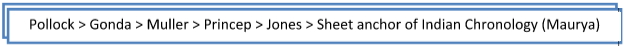
\includegraphics[scale=.45]{images/chap1-fig1.jpg}
\caption{Tracing Pollock’s\index{Pollock, Sheldon} bias}\label{chap1-fig1}
\end{figure}

Muller’s ‘Sheet-anchor of Indian chronology,’\index{Chronology}\index{Sheet Anchor of Indian Chronology@“Sheet Anchor of Indian Chronology”} close to hundred years after it was first conjectured by Jones, was subsequently christened ‘historically authenticated date of Chandragupta’ (Weber 1892:287) by Albrecht Weber in \textit{The History of Indian Literature} in which, of the seven occurrences of Candragupta\index{Candragupta}, in two of them, Jones’ conjecture can be seen becoming the basis for theorisations and/or conclusions on dating of Pāṇini,\index{Panini@Pāṇini} Kātyāyana\index{Katyayana@Kātyāyana} (Vararuci)\index{Vararuci} and Buddha-Gautama.\index{Buddha-Gautama}

Seven years after Weber’s declaration of Jones’ conjecture as ‘historically authenticated,’ Mabel Duff\index{Duff, Mabel}, in possibly the most extant colonial publication purely focused on Indian chronology—\textit{The} \textit{Chronology of India - From the earliest times to Beginning of Sixteenth century}—makes clear the reliance of colonial chronology of India on Muller’s ‘Sheet-anchor of Indian Chronology’, that is William Jones’ conjecture:

\begin{myquote}
“As is well known, the literature of the Hindus, extensive and valuable as it is, contains scarcely any works of historical character. For a trustworthy chronology of India, we are, therefore, mainly dependent on the testimony of coins and inscriptions. Where these fail us, as in the early history of the country, we are thrown back on conjectures and inferences which are always liable to be modified and upset by future discovery. To Sir William Jones we owe the identification of the Sandrokottos\index{Sandracottus/Sandrokottos} or Sandrokoptos of the Greek writers with Chandragupta, the founder of the Maurya dynasty, whose date, B.C. 315, affords a starting-point from which, with the aid of Singhalese and other Buddhist records eked out of Paranic tradition, it is possible to reconstruct with some degree of success an outline of the history of Upper India between the sixth and third centuries B.C.” 

~\hfill (Duff 1899:01)
\end{myquote}

In Duff’s chronological entries for Candragupta\index{Candragupta Maurya} Maurya and Gautama Buddha,\index{Buddha, the}\index{Buddha-Gautama} we find clear evidence of Roy’s statement that “the history of India that we know today has been constructed by counting backward and forward from these two sheet anchors” (Roy\index{Roy, Raja Ram Mohan} 2016a):

\begin{myquote}
“B.C. 315: Chandragupta establishes the Maurya dynasty at Pāṭaliputra. The chronology of this dynasty and that of Buddha's death are determined by the initial date assigned to this king (see B.C. 477).” 

~\hfill (Duff 1899:10)
\end{myquote}

\begin{myquote}
“B.C. 477: Buddha's\index{Buddha, the} death in the eighth year of Ajātaśatru,\index{Ajatasatru@Ajātaśatru} and calculated from the accession of Chandragupta, Maurya, which it preceded by 162 years.” 

~\hfill (Duff\index{Duff, Mabel} 1899:06)
\end{myquote}

For insider responses, while Roy’s work has largely been cited in the preceding portions, he is the latest in a line of listed insiders, some of whom have undertaken not only an exhaustive \textit{pūrva-pakṣa}\index{purvapaksa@\textit{pūrva-pakṣa}} but also provided \textit{uttara}-\textit{pakṣa},\index{uttarapaksa@\textit{uttara-pakṣa}} based on completely Indic sources, which include varying theories and chronologies. Some such key insiders include Troyer,\index{Troyer, M. Anthony} Narayana Sastry, M. Krishnamachariar,\index{Krishnamachariar, M.} D. R. Mankad\index{Mankad, D. R.}, Pandit Kota Venkatachelam, D.S. Trivedi\index{Trivedi, D. S.}, Kosla Vepa. In some of their proposed theories and chronologies, while one can still see differences and from which one can adduce that while the task of fixing India’s BCE chronology\index{Chronology} is far from complete, that task cannot be considered to have even been started, in objective earnest, if its foundational assumption, the ‘sheet-anchor’\index{Sheet Anchor of Indian Chronology@“Sheet Anchor of Indian Chronology”}, the C of our proposed ‘ABC of Indian chronology’ is not seriously reevaluated, whilst its credibility remains enshrined in NCERT textbooks, publications of our listed outsiders as well as others such as E. Sreedharan, who presents Elphinstone, in spite of his explicit rejection of several Hindu sources, as having “formed a high opinion of early Hindu civilization”(Sreedharan 2004:401) and remarks the following, about his method:

\begin{myquote}
“And now, without any difficulty, he fixed Chandragupta Maurya’s accession towards the end of fourth century BCE. Then counting backwards and forwards from this one point, he fixed the approximate dates of the royal dynasties mentioned in the \textit{Puranas}\index{purana@\textit{purāṇa}} from the Mahabharata\index{Mahabharata@\textit{Mahābhārata}}\index{Bharata war@Bhārat war} war to the Guptas\index{Guptas} in the fourth century AD. The chronological framework Elphinstone gave to ancient history is much the same as is generally accepted, though occasional modifications have been rendered by archeological discoveries of coins and inscriptions.” 

~\hfill (Sreedharan 2004:407) \textit{(Spelling and italics as in the Original)}
\end{myquote}

One wonders if it is to such Indians with outsider lens that M. Krishnamachariar almost prophetically refers, as “Professors of Indian History” in the following excerpt from his preface:

\begin{myquote}
“In the hands of many Orientalists, India has lost (or has been cheated out of) a period of 10-12 centuries in its political and literary life, by the faulty Synchronism of Candragupta Maurya and Sandracottus\index{Sandracottus/Sandrokottos} of the Greek works and all that can be said against the “\textit{Anchor-sheet of Indian Chronology}” has been said in this Introduction. In the case of those early European Orientalists, very eminent and respectable themselves, this thought of resemblance and historical synchronism was at least sincere; for it was very scanty material they could work upon. But for their successors in hierarchy who are mostly our “Professors of Indian History”, that have given a longevity and garb of truth to it by repetition, there is to my mind no excuse of explanation, if at all it be a confession of neglect and recognition of India’s glorious past in its entire truth.” 

~\hfill (Krishnamachariar\index{Krishnamachariar, M.} 1937:02)\textit{(Spelling and italics as in the Original)}
\end{myquote}

With elaborate refutation and evidence provided in the Introduction of his work, he further remarks:

\begin{myquote}
“Thus we see that Vincent Smith\index{Smith, Vincent} is the modern protagonist of this identity, the \textit{Anchor-sheet of Indian chronology.}\index{Chronology} It is he that is quoted and followed without enquiry by our Indian professors of history and it is this chronology that is and \textit{must be} taught in our schools. By sheer repetition by men in authority and in the works that emanate from them, the theory has become an axiom and rarely does any thought occur for any fair investigation. Day after day the assumed identity takes a firmer root and is considered a matter of senility or superstition to express a need for reconsideration. Hasty generalisations lead to prepossessions and it is rarely human to attempt to demonstrate their reality. It may appear therefore, a futile cry to seek to go behind these established opinions and to ask the reader to forebear and see for himself of the original bases of this theory, if after all, the narratives of the Purāṇas\index{purana@\textit{purāṇa}}, so honestly planned, are ‘pious frauds.’ For the vindication of the morality of our sages and the merit of our traditional lore, a lore adored by millions of Hindu India, an attempt must be made, be the effect as it may.” 

~\hfill (Krishnamachariar 1937:l xxxiv) \textit{(Spelling and italics as in the Original)}
\end{myquote}

Nearly 80 years after the above statement appeared in print, and close to 70 years after India became independent, many minds of her children as well as her textbooks of history across all levels are still not not freed from the clutches of colonial motives and narratives, whilst post-colonial scholars of Indology like Pollock\index{Pollock, Sheldon} seek to polarize her peoples using postmodern theories underpinned by motivated, colonial chronological conjectures.


\paragraph*{3.4.2.2 Debunking the 223-year-old conjecture: \hfill\break Past Attempts and a Recent One}

While M Krishnamachariar’s book was focused on Sanskrit literature and the sheet-anchor\index{Sheet Anchor of Indian Chronology@“Sheet Anchor of Indian Chronology”} was dealt with primarily in its introduction, Mankad’s\index{Mankad, D. R.} \textit{Puranic Chronology}\index{Chronology} and Kota Venkatachelam’s \textit{The Plot in Indian Chronology} deal exclusively with chronology from an insider’s point of view and while reaching different conclusions, they do a thorough \textit{pūrva-pakṣa}\index{purvapaksa@\textit{pūrva-pakṣa}} of Maurya synchronism and talk in one voice about the invalidity of the Candragupta\index{Candragupta} Maurya synchronism with Sandrokottos\index{Sandracottus/Sandrokottos}. Both Vepla and Roy refer to Kota Venkatachelam in their elaborations on this matter, however Dr. Roy, goes much further. After reaching the same conclusion as Venkatachelam about the implausibility of Sandrokottos being Candragupta Maurya with his evidence, he critiques though, Venkatachelam’s endorsement of Somayajulu’s proposals (that Devānāmpriya\index{Devanampriya Priyadarsi@Devānāmpriya Priyadarśī} Priyadarśī was not Aśoka\index{Asoka@Aśoka} Maurya but Aśokāditya\index{Asokaditya@Aśokāditya} and that Aśokāditya was another name of Samudragupta\index{Samudragupta}), on account of perceived lack of evidence. He then proceeds to first make compelling arguments himself to show “that the identification of Devānāmpriya Priyadarśī with Aśoka Maurya is not as sacrosanct as the modern historians would make us believe” (Roy\index{Roy, Raja Ram Mohan} 2016b) and then claims an original proposal, a result of his fourteen years research, that Kumāragupta-I\index{Kumaragupta-I@Kumāragupta-I} is Devānāmpriya Priyadarśī. The sheer impact that Dr. Roy's proposal could have on changing the face of India’s history as it is today, and the need for it to reach more scholars and citizens sensitive to India’s real history, compels the authors to reproduce a part of his conclusion here:

\begin{myquote}
“The identifications of Sandrokottos with Chandragupta-I and Devānāmpriya Priyadarśī with Kumāragupta-I, both of the Imperial Gupta dynasty, provide us the opportunity to reconstruct the history of India that better represents the evidence and is more faithful to the native traditions of India. In this chronological reconstruction we have a historical Vikramā\-ditya, the greatest hero of ancient India, whose death in 57 BCE is commemorated by starting the Vikrama era in 57 BCE. We also have Gautamīputra\index{Gautamiputra Satakarni@Gautamīputra Śātakarṇi} Śātakarṇi crushing Śakas in 78 CE which is celebrated by starting the Śaka\index{Saka@Śaka} era in 78 CE. Currently foreigners are given credit for instituting both of these important Indian eras by historians whose hearts are full of love for invaders and who specialize in making a mockery of our traditions.” 

~\hfill (Roy 2016c)
\end{myquote}

Whether or not Roy’s proposal that Kumāragupta-I\index{Kumaragupta-I@Kumāragupta-I} is a real breakthrough to solving the issue of the second sheet anchor\index{Sheet Anchor of Indian Chronology@“Sheet Anchor of India Chronology”}, there is little doubt that the first ‘sheet-anchor’ of Indian history was from its genesis, a motivated conjecture and while published challenges to it have existed starting from at least the mid-nineteenth century (Troyer)\index{Troyer, M. Anthony}, through the twentieth century (M. Krishnamachariar\index{Krishnamachariar, M.} (whose work was clearly known to Pollock\index{Pollock, Sheldon}), D. R. Mankad\index{Mankad, D. R.}, Kota Venkatachelam), up until contemporary times (Kosla Vepa, Roy\index{Roy, Raja Ram Mohan} himself), the quantity and quality of objective, unmotivated scholarship in mainstream Indology, on a topic as crucial as Chronology\index{Chronology} of India, has evidently been disproportionately sparse. Pollock could have been deemed only as guilty of the crime of not having addressed this issue as most of his innumerable predecessors, had he not proclaimed that staying true to insider sources was one of the key differentiating factors of his methods \textit{vis-à-vis} that of his predecessors, specifically colonial, never mind whether British or their Indian ‘Sepoy’, methods\endnote{ See Narayana Sastry (1916) Chapter 1 - Method of Investigation, for a brief appraisal on prevailing colonial methods.}. Given that Pollock’s scholarship is not known to have included considerations of conclusions from truly modern fields such as computerized simulations of literary astronomical references, one questions if Pollock has at least studied the literary evidence from truly traditional sources such as the wide range of texts Pandit Venkatachelam suggests (Venkatachelam 1953:14).



\section*{4. Pollock’s Theories Proceeding from his Chronological Framework}

Principal among Pollock’s assertions is that, at the onset of the first millennium C.E, Sanskrit transformed itself from being a sacred language to one of ‘literary and political expression.’ ‘Culture’, ‘power’, ‘pre-modernity’ and ‘cosmopolitan’ are the linchpins upon which his grand structures of the spread of Sanskrit as well as its domination are built. Pollock believes that ‘culture’ can be equated to its subset ‘language’ and a further subset, ‘literature’. Thus, for pre-modern India, \textit{kāvya},\index{kavya@\textit{kāvya}} with its history, nature and role becomes the pivotal basis. Pollock says his magnum opus \textit{The Language of Gods in the World of Men} could have carried an alternate sub-title “A Study of Big Structures, Large Processes, and Huge Comparisons,” (Pollock 2006:2) but his data set from which he leaps to imperious designs is so small, that surely his work could have been more aptly titled ‘A Study of Unsound Structures, Illogical Processes and Inaccurate Comparisons.’

\subsection*{4.1 Dismissal of the Oral Tradition and Emphasis on Writing}

With \textit{kāvya}\index{kavya@\textit{kāvya}} becoming such a focal point, Pollock\index{Pollock, Sheldon} considers aspects of it and at times, in a manner that disconnects very significant sections from the native points of view. While admitting that Western literary theory does not have a place for native concepts of \textit{pāramārthika}\index{paramarthika@\textit{pāramārthika}} and \textit{vyāvahārika}, Pollock astonishingly remarks that “One thing that could not be \textit{kāvya} is purely oral.” (Pollock 2006:3) Pollock boldly declares that \textit{kāvya} is defined in terms of the written, “practically if not explicitly,” (Pollock 2006:4) not just for the modern readers, but even the pre-modern. But, there has been no distinction at all between the written and the oral in traditional sources, be it Bhāmaha\index{Bhamaha@Bhāmaha} or Daṇḍin\index{Dandin@Daṇḍin} or Jagannātha\index{Jagannatha Panditaraja@Jagannātha Paṇḍitarāja} Paṇḍita and certainly not in the manner in which Pollock presents. For Pollock, “writing claims an authority oral cannot” (Pollock 2006:4) and this point is essential for his political lens to associate Sanskrit and its use with “privilege” and analyse the spread of the language. Pollock’s dating of \textit{kāvya} to last centuries BCE sits hand in glove with his claim that writing is also seen for the first time during the same period and the latter played a crucial role in the development of the former – “In short, the world of \textit{kāvya} was a world of literacy, and was so from the very first,” (Pollock 2006:87) “This phenomenology of the constitutive literacy of \textit{kāvya} is entirely consistent with the historical argument in favor of placing the beginnings of \textit{kāvya} after the technology of writing was disseminated in the subcontinent in the last centuries b.c.e.” (Pollock 2006:86)

 With this manifest bias towards the written and casual and startling dismissal of centuries of the oral, Pollock sets the stage for his key points – “the invention of literacy and growth of manuscript culture” (Pollock 2006:4) at the start of the Common Era which led to a complex socio-political structure through which Sanskrit began its reign across the Indian sub-continent. Ascribing enormous importance to the moment of introduction of writing, in fact, so much so that he believes a new word needs to be coined for the process, Pollock generously introduces us to “literization.”\index{literization} (Pollock 2006:4)

%\newpage

The import of writing in Pollock’s thesis of Cosmopolis\index{Sanskrit Cosmopolis} is also seen in its second major component – vernacularisation\index{vernacularisation}. Pollock believes that “We understand less of the history of culture in South Asia the less we understand of these dominant conceptions, including the essentialization of literature and the primacy granted to writing in the constitution of literature,” (Pollock 2006:5). Thus, writing and consequently, the new forms of Sanskrit literature as well as socio-political transformations it heralded during the beginning of CE, set the norm for the commencement of literature in the vernacular languages as well. But, if one were to momentarily admit his supposition, the following statement, in light of the monumental significance of the historical dating of Candragupta\index{Candragupta} Maurya, at once confutes his chronological placement of the introduction of writing and \textit{kāvya}\index{kavya@\textit{kāvya}} in India –

\begin{myquote}
“Our ability to trace the lineaments of the expansion of Sanskrit’s social and discursive domain, and to understand something of the new cultural political order this generated, takes on an altogether different degree of historical precision once we enter the age of writing. This commenced around the middle of the third century b.c.e. with the records issued by Aśoka\index{Asoka@Aśoka}, the third overlord of the Maurya dynasty (320–150 b.c.e.). This has long been known. An emerging scholarly consensus, however, now regards the Brahmi syllabary, the first South Asian writing system (and the parent script for almost every other writing system in southern Asia), as the deliberate creation of Aśoka’s chancery for the promulgation of his edicts\index{Asokan edicts@Aśokan edicts} on moral governance (in both the epigraphical idea itself and some of its formulaic language Aśoka was imitating Achaemenid practices)” 

~\hfill (Pollock\index{Pollock, Sheldon} 2006:59)
\end{myquote}

The waves from the mammoth, pervasive ramifications of this single colonial dating artifact of Maurya Candragupta seems to never ebb.



\subsection*{4.2. Invention of \textit{Kāvya}}

Pollock, at the very outset of \textit{The Language of Gods in the World of Men} clearly sets out that his aim is to study the culture-power practices of Sanskrit without agonizing over the details of whether the practices indeed form the right set of questions to explore. He feels the use of \textit{saṁskṛti}\index{samskrti@\textit{saṁskṛti}} is itself unattested in pre-modern times and prefers to use Cosmopolis, even though the latter may not be entirely suitable to describe the set of conditions he considers, and counter-examples can indeed be found to contest his claims. In the process of building this timeline for the invention of \textit{kāvya}\index{kavya@\textit{kāvya}} and lay the basis for the construct of Cosmopolis\index{Sanskrit Cosmopolis}, Pollock dates crucial milestones in Indian literary and socio-political history in a manner which is far removed from traditional chronology\index{Chronology} and expounds the conditions and implications of his timeline. Some of these key milestones are below.

\vspace{-.4cm}

\subsubsection*{4.2.1 Dating of \textit{Mīmāṁsāsūtra}\index{Mimamsa@Mīmāṁsā}}

In setting the tone for the dramatic nature of the formation of the Cosmopolis, Pollock\index{Pollock, Sheldon} believes that “social monopolization and discursive ritualization” (Pollock 2006:51) were themain features of the language and the community which it represented in the centuries of BCE. Pollock cites Jaimini’s\index{Jaimini}\index{Jaimini Sutra-s@Jaimini Sūtra-s} \textit{Mīmāṁsāsūtra} as being the authoritative text on the matter and places it in the last centuries (2 or 3) BCE. He says the work was influenced by the spread of Buddhism\index{Buddhism} and hints at a causal link between the two –

\begin{myquote}
“There is good reason to believe that the reflexivity, even anxiety, about Vedic authority evinced in the work, of which the restriction on access to the corpus and its language is only one (if a decisive) component, would have been unthinkable in the absence of the broad religious and social critique that Buddhism had enunciated in the preceding two centuries and the ‘disenchantment of the world’ that critique had signaled. But if the reflexivity of the \textit{Mīmāṁsāsūtra} was new, relatively speaking, the restrictions it promulgates were not,” 

~\hfill (Pollock 2006:40)
\end{myquote}

Pollock, from the entire discourse chooses to focus primarily on the \textit{Adhikāra}\index{adhikara@\textit{adhikāra}} chapter of \textit{Pūrvamīmāṁsa} and despite its rather unremarkable position in the work, is convinced the chapter is indicative of the social conditions of the day. Pollock believes that Sanskrit was confined in its usage only for sacred purposes and hence, restrictions on who could use it were built into the language. He thus reduces the conditions that existed for thousands of years before CE to one where the Vedic circle alone exercised monopoly over the use of Sanskrit for ritualistic purposes. Curiously, Pollock admits that the conditions that existed may have been less rigid, and acknowledges the same from Jaimini’s work (Pollock 2006:41).

But, it is only in briefly considering alternate pictures and dismissing them that he betrays his motives. The chronological placing of Jaimini’s\index{Jaimini}\index{Jaimini Sutra-s@Jaimini Sūtra-s}\index{Mimamsa@Mīmāṁsā} \textit{Mīmāṁsasūtra} this way, along with Buddha himself during the 5 century BCE is preeminent for Pollock’s premise of Buddhism being the influential factor to which the Vedic society was necessitated to provide a response.

Positioning Buddhism as the silver bullet that saved the ancient Indian from the clutches of Vedic oppression and creating a dichotomy between the two is a recurrent theme of Pollock’s oeuvre,

\begin{myquote}
“The most important of them for our purposes here are embodied in the language theory and practices of early Buddhism, though these were in fact only part of a larger process, a transvaluation\index{transvaluation} of values, that occurred in the last centuries before the Common Era. This stood in radical opposition to the naturalism of the \textit{vaidika} thought world. The new conventionalism came to have application not only to individual psychology but to the social world at large and, more important in the present context, to language. In light of these broad tendencies, there was every reason for Buddhism\index{Buddhism} to reject Sanskrit in the course of its confrontation with the social-religious practices for which Sanskrit was the principal vehicle,” 

~\hfill (Pollock\index{Pollock, Sheldon} 2006:51)
\end{myquote}

After having repeatedly highlighted the challenge and radical departure the rise of Buddhism posed to the \textit{vaidika} world, Pollock expresses wonder that by the turn of the millennium, Buddhists have abandoned their use of Pāli and Prakrit exclusively and resorted to Sanskrit,

\begin{myquote}
“The fact that many Buddhist communities in the north of the subcontinent abandoned their long-standing language pluralism in favor of Sanskrit, the language they had rejected for centuries, therefore awaits better explanations.” 

~\hfill (Pollock 2006:59)
\end{myquote}

He does not give any credence to the possibility that the two \textit{dharma} based faiths, over the course of centuries of simultaneous existence, could have seen a detente and tempering of exchanges and is in fact, dismissive of more reasonable and guileless accounts of history and mutual influence between the two. Especially given the challenge to the colonial Indological dating of the Mauryan empire, Pollock’s thesis stands on fragile ground:

\begin{myquote}
“The standard account of Sanskrit cultural-political history purports to explain these developments by postulating a “resurgence of Brahmanism” leading to a “reassertion” or “revival” of Sanskrit as the language of literature and administration after the Maurya period. The more plausible interpretation is that a new cultural-political formation, a Sanskrit cosmopolitan formation, was on the point of being invented. The textbook narrative posits the resurgence of a community we have no reason to believe was in need of resurgence; it assumes a reassertion at the expense of Buddhism\index{Buddhism}, which in fact hardly suffered a subsequent decline (quite the contrary, it expanded markedly); it asks us to believe in the revival of cultural forms that cannot be shown to have preexisted in the first place.” 

~\hfill (Pollock 2006:74)
\end{myquote}

One wonders at the motives behind such purposeful undervaluing of alternate, plausible accounts.

\vspace{-.4cm}

\subsubsection*{4.2.2: Pollock’s Dating of Vālmīki\index{Valmiki@Vālmīki} \textit{Rāmāyaṇa}\index{Ramayana@\textit{Rāmāyaṇa}} and its Implications}

\vspace{-.2cm}

Pollock in his \textit{The Language of Gods in the World of Men} repeatedly paints a picture of Sanskrit having no other primary function apart from the sacerdotal in BCE and that the language spread rapidly once it was freed from this role —

\begin{myquote}
“Once Sanskrit emerged from the sacerdotal environment to which it was originally confined, it spread with breathtaking rapidity across southern Asia.” 

~\hfill (Pollock\index{Pollock, Sheldon} 2006:14)
\end{myquote}

but, during the last two centuries of BCE and at the dawn of the new millennium, Sanskrit acquired a “new sociology and politicization of the language,” (Pollock 2006:12) even as Pollock attributes a role to the “western Asian and central Asian peoples” (Pollock 2006:12) while referring to the Śakas. This is representative of his typical, biased attribution of social change and innovation to the good outsider, be it the Śakas\index{Saka@Śaka} or the Greeks. Pollock confidently refers to \textit{kāvya}\index{kavya@\textit{kāvya}} as an invention of the period of the commencement of the Cosmopolitan era, along with its subset \textit{praśasti}\index{prasasti@\textit{praśasti}} and together, they drove forward the Cosmopolis\index{Sanskrit Cosmopolis} construct.

Highlighting the features of \textit{kāvya} and how different it was from every literary form prior to it, Pollock astonishingly states that “\textit{kāvya} was almost certainly composed and circulated (though not typically experienced) in writing” (Pollock 2006:13), in spite of there being no evidence to this statement and that it was “a new phenomenon in Indian cultural history when it first appeared a little before the beginning of the Common Era” (Pollock 2006:13). Pollock then makes a second startling statement regarding the dating of the first poem Vālmīki\index{Valmiki@Vālmīki} \textit{Rāmāyaṇa},\index{Ramayana@\textit{Rāmāyaṇa}} placing its creation in the first two centuries before the advent of the CE

\begin{myquote}
“In reflexively framing its own orality in a way that would be impossible in a preliterate world, and in doing so around the narrative of human response to problems of a human scale, the \textit{Rāmāyaṇa} account captures some central features of the new expressive form that was \textit{kāvya.}”\index{kavya@\textit{kāvya}} 

~\hfill (Pollock 2006:13)
\end{myquote}

\newpage

His dating of Vālmīki \textit{Rāmāyaṇa} is especially crucial, for it reinforces his idea that the social order was primed for change -

\begin{myquote}
“The \textit{Vālmīki Rāmāyaṇa}, which both literary tradition and the text itself regard as the first Sanskrit \textit{kāvya}, represented an entirely new genre in Indian literary history, and its reflexive understanding of the social and discursive peculiarities of the language it employed became possible only at a moment that marked the beginning of a new cultural order.” 

~\hfill (Pollock\index{Pollock, Sheldon} 2006:45)
\end{myquote}

Pollock withal maintains that Sanskrit never fulfilled a role of being used for everyday communication by citing that there has been no evidence to the contrary -

\begin{myquote}
“Sanskrit probably never functioned as an everyday medium of communication anywhere in the cosmopolis\index{Sanskrit Cosmopolis}—not in South Asia itself, let alone Southeast Asia— nor was it ever used (except among the literati) as a bridge- or link- or trade language like other cosmopolitan codes such as Greek, Latin, Arabic, and Chinese.” 

~\hfill (Pollock 2006:14)
\end{myquote}

Given this ill-founded and outrageous assumption of Sanskrit’s role and use, the dating of Vālmīki \textit{Rāmāyaṇa} bears greater significance when Pollock says the following:

\begin{myquote}
“It is significant that, with the exception of the Rāmāyaṇa\textit{,} no remains of a nonsacral, this-worldly Sanskrit are extant from the early epoch of literacy (from the third century b.c.e to, say, the first century c.e.), when, as some believe, Sanskrit was still supposed to have been an everyday idiom, whereas vast amounts of such Sanskrit are available from the later period when Sanskrit ‘had ceased to be truly a current language.’” 

~\hfill (Pollock 2006:48)
\end{myquote}

This is indeed dubious methodology by the author, for there is no evidence for his claims regarding the conditions that existed in the last millennium BCE, of Sanskrit being restricted to ritualistic practices alone, with its use confined to the Vedic practitioners and the social conditions representing the same. Pollock paints a picture of contrast for the use of Sanskrit in BCE and in the first millennium CE, with the former being one of strict use of the language for sacerdotal alone (no evidence cited for these conditions), and against this background, he aims to show that the language became one used for \textit{kāvya}\index{kavya@\textit{kāvya}} and to capture emotional content.

Moreover, with the traditionalist’s dating of \textit{Rāmāyaṇa},\index{Ramayana@\textit{Rāmāyaṇa}} it becomes manifestly clear that \textit{kāvya} was not the invention of the CE but a form of literature that has existed for centuries prior! And, as Pollock himself maintains, Vālmīki\index{Valmiki@Vālmīki} \textit{Rāmāyaṇa} represents the commencement of a genre that marked one of the greatest achievements of the Sanskrit language. But, with the timeline in which the insider places \textit{Rāmāyaṇa}, Pollock’s\index{Pollock, Sheldon} premise of it characterizing the social order and period of innovation in the last centuries of BCE reduces to disannulled conjectures. Against the chronological backdrop of \textit{Rāmāyaṇa}, Pollock’s repeated dinning of the farcical idea of \textit{kāvya} being invented at the turn of the CE and an entire civilization consumed with no other goals except ritualistic ones seems highly suspect and puerile. Vālmīki \textit{Rāmāyaṇa} has been rightly hailed as one of the greatest epics of our culture, simultaneously being a representation of the Indian ethical mind and a touchstone for \textit{kāvya} until the modern day. Pollock’s discordant dating of the epic and hence, the very commencement of \textit{kāvya}, thus strikes oppugnant notes with the insider accounts.

Having set aside analytical terms from the tradition itself such as \textit{saṁskṛti},\index{samskrti@\textit{saṁskṛti}} Pollock’s unsubstantiated statements of associating \textit{kāvya} exclusively with the written and his placing its invention close to the start of CE feels more a deliberate attempt at legitimizing his Sanskrit Cosmopolis\index{Sanskrit Cosmopolis} theory rather than the latter idea being driven by facts. Pollock further charges Sanskrit grammar to be an instrument of power of the language, by insisting that “a vision of grammatical and political correctness—where care of language and care of political community were mutually constitutive—was basic to the cosmopolitan ethos from the very beginning” (Pollock 2006:15). “Sanskrit philology was a social form as well as a conceptual form, and it was inextricably tied to the practices of power.” (Pollock 2006:15).

\vspace{-.3cm}

\subsubsection*{4.2.3: Pollock’s Dating of Pāṇini, Patañjali\index{Patanjali@Patañjali} and its Implications}

\vspace{-.2cm}

Pollock places the landmark \textit{Aṣṭādhyāyi}\index{Astadhyayi@\textit{Aṣṭādhyāyi}} of Pāṇini around 3 or 4 century BCE, and this only reinforces his picture of a society where grammar was a tool to preserve the purity of the language and restrict those who could participate in its use. Pollock also places Patañjali’s \textit{Mahābhāṣya}\index{Mahabhasya@\textit{Mahābhāṣya}} into the first centuries of CE and highlights its use for the sacred:

\begin{myquote}
“In the \textit{Aṣṭādhyāyi}, this sacerdotal function characterizes both registers of the language: on the one hand, the idiom actually used for the Vedic texts themselves, what Pāṇini\index{Panini@Pāṇini} calls chandan, verse, or better, “the Verse”; on the other, the rigorously normative idiolect restricted to (Vedic) pedagogical environments, which he calls \textit{bhāṣa}, speech. That both had largely sacral associations as late as the beginning of the Common Era is shown in Patañjali’s \textit{Mahābhāṣya}, the \textit{Great Commentary} on Pāṇini’s grammar.” 

~\hfill (Pollock 2006:46)
\end{myquote}

Pollock\index{Pollock, Sheldon} holds even the \textit{Mahābhāṣya} to the same line of thinking, in underscoring the role it played to ensure the use of the language remained primarily for ritualistic and religious purposes

\begin{myquote}
“Not all of these reasons may be entirely clear to us, but there can be little doubt that for Patañjali, principal heir and final arbiter of the \textit{vaidika} grammatical tradition, the purposes of Sanskrit language analysis were more or less exclusively tied to sacred performance and to the pedagogical practices, both social and discursive, pertaining to knowledge of the sacred.” 

~\hfill (Pollock 2006:47)
\end{myquote}

Pollock sets Kātyāyana’s\index{Katyayana@Kātyāyana} time to be in between that of Pāṇini and Patañjali.

As is seen from some traditional sources, Pollock’s dates of these three crucial figures do not concur with the traditional accounts. It’s vitally important for Pollock to date these landmark texts and luminaries close to the beginning of CE for it highlights the divergence the socio-political conditions of the period are set to experience, with the ‘invention of \textit{kāvya}’ in the close to the first millennium of CE. Given Pollock’s constant reiteration of Sanskrit being confined to liturgical purposes alone for millennia, he builds a case for \textit{vyākaraṇa}, being a limb of the \textit{Veda}, to be an instrument that enforced and perpetuated the exclusive monopolization of Sanskrit. It is bemusing indeed, even a tad absurd, that a language and its grammar can possess the power to exercise such domination over every strata of the socio-political conditions of a culture for millennia and one feels perhaps Pollock’s scrutiny of the very composition of the term Saṁskṛtam and \textit{dévabhāśa} crosses over into the realm of incredulity.

\vspace{-.5cm}

\subsubsection*{4.2.4. \textit{Kāvya praśasti}\index{kavya@\textit{kāvya}}\index{prasasti@\textit{praśasti}} and Cosmopolis\index{Sanskrit Cosmopolis}}

\vspace{-.3cm}

Having painted a picture where the socio-political conditions have been dominated for centuries by ritualization and monopolization, Pollock maintains that it was due to the “innovative force” provided by the outsider i.e. the Śakas,\index{Saka@Śaka} whom he places during the period 100 BCE - 400 CE, that the breach against the authoritarian old order was made. In quintessential style, Pollock\index{Pollock, Sheldon} believes that Sanskrit was appropriated by the Śakas — initiated by Rudradāman\index{Rudradaman@Rudradāman} — for public display of political power, leading to the creation of the Indian panegyric \textit{praśasti} and literature itself – “What had now begun, however, was not only \textit{praśasti} but also the genus of which that discourse is a species. In other words, what began when Sanskrit escaped the domain of the sacred was literature,” (Pollock 2006:74). With this new mantle, Sanskrit descended and travelled freely in the world of men, without being tied down to a region or liturgical purpose alone.

Attributing any new impetus or socially liberating role to forces outside the Vedic order is a chief hallmark of Sheldon Pollock’s work and his bias. Be it Buddhism\index{Buddhism} in the socio-religious domain or the Śakas in the socio-political world, he portrays an image of Sanskrit being freed from the clutches of the dominating, oppressive traditional order. In this portrayal, written works and \textit{kāvya} and \textit{praśasti} and liberating Buddhist ideals become \textit{ne plus ultra} while oral works and grammar and Vedic order get rendered as organs of hegemony. And Pollock even points to a possible relationship and similarities between the appropriation of Sanskrit by the Śakas and the Buddhists (Pollock 2006:72).

Chronologically, having Buddhist influence contemporaneous with the Śakas leads his premise of the conditions of the day set for a mammoth change:

\begin{myquote}
“Earlier scholars may have been right to argue that the new overlords only consecrated the vogue of literary Sanskrit and did not create it, though the evidence to prove this conclusively does not exist. A caution has been raised against adopting any mechanistic model and in favor of viewing the factor of political change as mere concomitance (and, we are rightly warned, “concomitance is not causality”), yet the synchrony of the two events is striking, and it may ultimately prove correct to locate in the Śaka\index{Saka@Śaka} practices a truly ‘innovating force.’” 

~\hfill (Pollock 2006:72)
\end{myquote}

But, Pollock not only throws caution to the wind but goes ahead in his quest to find a grand role for Sanskrit, if only based on grander and one must add ludicrous assumptions.

Pollock\index{Pollock, Sheldon} is dismissive of accounts that dispute his thesis –

\begin{myquote}
“The standard account Sanskrit cultural-political history purports to explain these developments by postulating a “resurgence of Brahmanism” leading to a “reassertion” or “revival” of Sanskrit as the language of literature and administration after the Maurya period. The more plausible interpretation is that a new cultural-political formation, a Sanskrit cosmopolitan formation, was on the point of being invented. The textbook narrative posits the resurgence of a community we have no reason to believe was in need of resurgence; it assumes a reassertion at the expense of Buddhism\index{Buddhism}, which in fact hardly suffered a subsequent decline (quite the contrary, it expanded markedly); it asks us to believe in the revival of cultural forms that cannot be shown to have preexisted in the first place. Sanskrit of the kind under discussion had not died; rather, it had not yet been born, at least not for the uses to which it was about to be put—\textit{laukika},\index{laukika@\textit{laukika}} or this-worldly, uses, such as political discourse, beyond the domain of the liturgy and its sacral auxiliaries.” 

~\hfill (Pollock 2006:74)
\end{myquote}

His rejection of the more plausible standard account feels labored, given his penchant for downplaying any transformative causes from within the \textit{dharma} based social system. A dynamic social order, which innovated and produced works, be it in literature or the sciences, finds no place or even mere consideration in Pollock’s theorization. Chronologically, if one were to admit native sources and data, one sees an absence of a design that could lead to Pollock’s account. The dating of \textit{kāvya}\index{kavya@\textit{kāvya}} itself, with the timeline of \textit{Rāmāyaṇa},\index{Ramayana@\textit{Rāmāyaṇa}} places the impact of its creation in an asynchronous manner with respect to Pollock’s “moment of rupture” (Pollock 2006:73). One feels that the traditional dating of Buddha\index{Buddha, the} and rise and decline of Buddhism lends itself more reasonably to not only the enormous positive influence as well as the mutual acceptance it shared with \textit{sanātana dharma}-based beliefs but also, the eventual embracing of Sanskrit itself by Buddhist practitioners. Pollock’s argument for Buddhism\index{Buddhism} “appropriating” Sanskrit words including \textit{dharma} and \textit{sūtra} and the eventual rejection of Prakrit for the new, transformed, liberated Sanskrit during the start of CE wears the colours of convoluted and fanciful theorization more than those of equitable justification.

If the creation of \textit{praśasti},\index{prasasti@\textit{praśasti}} whose style is defined by Pollock as “the standard \textit{praśasti} style: the fixing of genealogical succession, the catalogue of kingly traits of the dynasty, and a eulogy of the ruling lord,” (Pollock\index{Pollock, Sheldon} 2006:119) marks the heralding of the cosmopolitan order of Sanskrit, Pollock’s characterization of the new features of the language are dramatic. With his unconvincing dismissal of standard theories and use of contestable chronological data to build a case, he declares:

\begin{myquote}
“Many uncertainties continue to obscure our insight into the origins of the Sanskrit cultural-political formation, the agents involved, and their social goals. But at least the fact that this formation \textit{did} begin should now be beyond dispute.” 

~\hfill (Pollock 2006:74)
\end{myquote}

In tracing the attributes of this momentous formation, Pollock focuses on the relationship between \textit{kāvya}\index{kavya@\textit{kāvya}} and \textit{rājya}, with \textit{praśasti} being representative of power and a “new politics of culture and culture of politics” (Pollock 2006:73). The first of these attributes is the role of Sanskrit in the new linguistic space it entered. Pollock believes that Sanskrit assumed a position unique from the regional languages, which were more locally tied, as against the former –

\begin{myquote}
“Considered carefully, these interactions reveal much about both the general character of the cultural political identity of the cosmopolitan polity and the particular kind of tasks that Sanskrit—and never the vernacular—was empowered to execute, precisely as envisioned by the theory of literary language.” 

~\hfill (Pollock 2006:115)
\end{myquote}

The interaction between Sanskrit and regional languages assumes a dichotomous role in Pollock’s work, with the latter increasingly giving rise to literature and the former restricted to courtly use and symbolizing power –

\begin{myquote}
“Just this division of labor was to be replicated with respect to the languages of Place: Sanskrit would monopolize all ideational and expressive functions in inscriptional and other written discourse while assigning to regional languages the quotidian status and function they had in everyday life,” 

~\hfill (Pollock 2006:118)
\end{myquote}

Pollock characterizes this as complex interaction between the two sets which led to increasing vernacularisation\index{vernacularisation} in the second millennium of CE, giving him the platform to introduce parallels with European vernacularisation as well.

Secondly, Pollock states that, as “the language of royal encomium,” (Pollock\index{Pollock, Sheldon} 2006:115) Sanskrit had clear objectives and reduces its aesthesis to one of politically motivated expression. One wonders at this bizarre characterization as even a casual survey of works produced in the language over the past two thousand years shows not only the peaks they aimed and reached but the very range has been among the broadest! What is more remarkable than Pollock’s cosmopolitan thesis is his method of only considering instances that purportedly defend his projections. One finds it hard to reckon such methodology when what is at stake with his conjectures is the very role and nature of Sanskrit over many centuries –

\begin{myquote}
“It is not necessary, even were it possible, to provide a complete survey of the institutionalization of the Sanskrit political idiom for the vast space-time of the cosmopolis.\index{Sanskrit Cosmopolis} Concentrating on a few exemplary cases will suffice to suggest the historical rhythm and spatial extent of the dissemination of Sanskrit, as well as the specific functions Sanskrit executed to the exclusion of other available codes.” 

~\hfill (Pollock 2006:115)
\end{myquote}

And even when one finds examples readily to disprove his thesis, Pollock is quick to dismiss them by focusing on selective parts of the case. Illustrating through the choice of language in the courts of Ikṣvāku\index{Iksvakus@Ikṣvākus} and Vākāṭaka\index{Vakataka@Vākāṭaka} rulers, Pollock highlights how Prakrit and Sanskrit interacted with each other in a manner that justifies his theorization but when it comes to the case of Pallavas\index{Pallavas}, while Pollock admits that indeed there is evidence for Sanskrit being used as a communicative medium for everyday life during their rule, there is no example of the regional languages being employed in a role similar to that of \textit{praśasti}\index{prasasti@\textit{praśasti}} –

\begin{myquote}
“While examples exist in earlier Pallava\index{Pallavas} records of Sanskrit being used to document the everyday world—a function that would become increasingly rare wherever it could be relegated to the vernacular—none exists where the everyday language is allowed to do the work of Sanskrit in a \textit{praśasti:}\index{prasasti@\textit{praśasti}} the literary work of interpreting and supplementing reality and revealing it in its truth.” 

~\hfill (Pollock 2006:122)
\end{myquote}

If one were to accept \textit{selection bias} and \textit{proof by example} as chief characteristics of Pollock’s modus operandi, certainly one sees the natural emergence and defense of the Cosmopolis\index{Sanskrit Cosmopolis} construct of Sanskrit.

\newpage

Pollock’s\index{Pollock, Sheldon} use of Cosmopolis to describe the transformation of Sanskrit is peculiar, as he attributes to a language, a uniquely chosen subset of culture, features and designs that are coloured with the lens of power. On the other hand, there have been writers from the insiders’ part of the spectrum who have truly brought out the import of the word Cosmopolis in a manner that not only ascribes proper place to the lenses of power and rule, and yet, refrained from projecting outré intentions to a language! D. R. Mankad\index{Mankad, D. R.} characterizes Samudragupta’s\index{Samudragupta} rule as being one where the ruler’s outlook helped create a “cosmopolitan and vigorously practical religion” (Mankad 1951:279), while comparing the roles of Maurya Aśoka\index{Asoka@Aśoka} and Samudragupta in propagating their respective beliefs. Understanding the evolution of socio-political and cultural conditions from this basis lends itself naturally to an understanding of how Sanskrit established its presence across the sub-continent as against harping on outlandish and even suspect constructs.


\vspace{-.3cm}

\section*{5. Conclusion}

Among Pollock’s extensive scholarship, characterized at times by Daedalian writing, one deciphers not only distinctive patterns of analysis but also the inclination towards asking the most ambitious of questions related to the domain. In the process of answering them, Pollock’s assumptions and methodology reveal his bias — some, his own and some, inherited from his colonial predecessors — as well as his proclivity to define the pre-modern conditions of India in a manner that lets him make grand comparisons that adroitly pit one Indological system against another. Thus, comparison is a key trait of Pollock’s analytical approach and as he himself states in \textit{Comparison Without Hegemony}, the basis of comparison is chronology\index{Chronology} -

\begin{myquote}
“Not only should chronology be central to comparative intellectual -historical practice—which is not the same thing as comparative philosophy—but no given model of intellection can be held to be universal. Observing this limit, I argue below, is critical if comparativism is to be saved from itself. It is vitally important, thus, that the synchronicity grounding comparative intellectual history contain no necessary content of this or any other sort.” 

~\hfill (Pollock 2010:10)
\end{myquote}

\newpage

With this centrality accorded to chronological data, it becomes all the more imperative to ensure one is on firm ground before positioning one’s theories, especially those that aim to build grand structures. Lamentably, Pollock’s\index{Pollock, Sheldon} chronology of key Indological events is a small, spartan bag comprising of inherited assumptions and convenient placements of key data, perhaps to create a synchronicity where none naturally exists, and is woefully short of even a semblance of a stable foundation. Be it his dating of the invention of \textit{kāvya}\index{kavya@\textit{kāvya}} or the composition of \textit{Rāmāyaṇa}\index{Ramayana@\textit{Rāmāyaṇa}} or key figures such as Buddha\index{Buddha, the}\index{Buddha-Gautama} Gautama and even Pāṇini,\index{Panini@Pāṇini} there is little uncontested ground for Pollock to make sweeping generalisations regarding fundamental, formative elements of Indian civilisation and culture. It is not the façade wearing Sanskrit lover who bears the burden of the weight of these vexing and exasperating theories but the native who faces the reality of being on the side which paid the highest possible price to the plunderers for political freedom.

Recognizing the criticality of chronological data to Pollock’s theorisation, we have in the course of this paper aimed to address questions including “Does tradition disagree with some of the dates he assigns? Which ones and with what evidence or logic do traditional scholars disagree with SP? Are there other examples in his work that show bias?” as well as identify main inconsistencies in Pollock’s data by firstly, reconstructing his chronology and checking them for the same; secondly, comparing his data with that from the outsider and insider realms; and thirdly, studying Pollock’s theories proceeding from his chronology which address larger concerns, with potentially greater consequences for his models and conclusions. While the authors have limited their focus to BCE part of chronology and therein identifying potentially the most important chronological epochs – the ABC of Indian chronology – Tables 1 and 2 are not limited to BCE, in order to enable ease of reference for any future \textit{pūrva-pakṣa}\index{purvapaksa@\textit{pūrva-pakṣa}} that chooses to focus on the CE portions of Pollock’s\index{Pollock, Sheldon} work. We have addressed in the paper at several levels the chronological placement and use of key texts over the last four centuries – by examining the very basis of colonial Indology, how texts get interpreted in terms of neo orientalist tools of power and culture, especially in the works of Pollock. We have not addressed vernacular literary texts in as much detail as we would have liked, as we believe it deserves a more detailed analysis and is given a basis in the present paper.

In the process of working on this paper, what clearly stood out from the score and deeply impacted us authors are the works of several native voices that have, with clarity and depth and exigency repeatedly tried to ensure the truth survived, in spite of the legion of assaults brought down upon them. The willful propagation of fallacious chronological data has, as shown in this paper, been the keystone for and symbolic of, the perpetuation of imperialistic design. Modern/ pre-modern, colonial/postcolonial theories of Indology will truly be insightful only when the very basis of these paradigms is carefully re-examined, the age old, deeply entrenched bias admitted, and the foundation rewritten without the utilitarian and detestable intentions of the coloniser or his native sepoy. And that process can begin to be effective only when the indigene is given, or he takes, his rightful place at the table, for it is verily his most deep-rooted, cherished creations and canons that have been set on the balance for judgment.


\section*{Appendix A -- Sheldon Pollock’s Chronology\index{Chronology} Reconstructed from His Scholarship}

\textbf{Table 1 (continued)}

\begin{longtable}{|l|p{2.5cm}|p{2.5cm}|p{2.2cm}|}
\hline
S No. & \multicolumn{2}{c|}{Epoch} & Source \\
\hline
  & Period (CE) & Detail &   \\
\hline
70 & 900 – 1200 & Cōḻas & Pollock 2006:597 \\
\hline
71 & 900 – 1300 & Yādavas of Dévagiri & Pollock 2006:597 \\
\hline
72 & 900 – 1400 & Angkor & Pollock 2006:597 \\
\hline
73 & 960 – 1200 & Kalyāṇa Cāḷukyas & Pollock 2006:597 \\
\hline
74 & 1000 – 1300 & Caulukyas (\textit{sic}) of Gujarat & Pollock 2006:597 \\
\hline
75 & 1000 – 1300 & Hoysaḷas\index{Hoysalas} & Pollock 2006:597 \\
\hline
76 & 1011 – 1055 & King Bhoja\index{Bhoja} & Pollock 2006:105 \\
\hline
77 & 1100 – 1400 & Kākatīyas\index{Kakatiyas@Kākatīyas} & Pollock 2006:597 \\
\hline
78 & Early 12th   century & Serpentine Scimitar of King Udayāditya & Pollock 2006:Cover \\
\hline
79 & 12th century & Vāgbhaṭa & Pollock 2006:112 \\
\hline
80 & 1340 – 1565 & Vijayanagara & Pollock\index{Pollock, Sheldon} 2006:597 \\
\hline
\end{longtable}

\textbf{Table 2: Sheldon Pollock’s Chronology\index{Chronology} of texts reconstructed from Pollock’s book \textit{A Rasa\index{rasa@\textit{rasa}} Reader: Classical Indian Aesthetics}}

\begin{longtable}{|l|p{1.1cm}|p{1.98cm}|p{1.98cm}|p{1.98cm}|}
\hline
S No. & Dating (CE) & Transliterated Sanskrit Name & Author (as per Pollock) & Pollock’s English Name \\
\hline
1 & 300 & \textit{Nāṭya-śāstra} & Bharata & Treatise on Drama \\
\hline
2 & 650 & \textit{Kāvyālaṅkāra}\index{Kavyalankara@\textit{Kāvyālaṅkāra}} & Bhāmaha\index{Bhamaha@Bhāmaha} & Ornament of Poetry \\
\hline
3 & 700 & \textit{Kāvyādarśa}\index{Kavyadarsa@\textit{Kāvyādarśa}} & Daṇḍin\index{Dandin@Daṇḍin} & Looking Glass of Poetry \\
\hline
4 & 800 & \textit{Kāvyālaṅkāra-sāra-saṅgraha}\index{Kavyalankarasarasangraha@\textit{Kāvyālaṅkārasāra-saṅgraha}} & Udbhaṭa\index{Udbhata@Udbhaṭa} & Essential Compendium of the Ornament of Poetry \\
\hline
5 & 825 & \textit{Nāṭya-śāstra-vyākhyā}\index{Natyasastravyakhya@\textit{Nāṭya-śāstra-vyākhyā}} & Bhaṭṭa Lollaṭa\index{Bhatta Lollata@Bhaṭṭa Lollaṭa} & Commentary on the Treatise on Drama \\
\hline
6 & 850 & \textit{Kāvyālaṅkāra} & Rudraṭa\index{Rudrata@Rudraṭa} & Ornament of Poetry \\
\hline
7 & 859 & \textit{Nāṭya-śāstra-vyākhyā}\index{Natyasastravyakhya@\textit{Nāṭya-śāstra-vyākhyā}} & Śrī Śaṅkuka\index{Sri Sankuka@Śrī Śaṅkuka} & Commentary on the Treatise on Drama \\
\hline
8 & 875 & \textit{Dhvanyāloka}\index{Dhvanyaloka@\textit{Dhvanyāloka}} & Ānandavar\-dhana\index{Anandavardhana@Ānandavardhana} & Light on Implicature \\
\hline
9 & 900 & \textit{Laghu-vṛtti}\index{Laghuvrtti@\textit{Laghu-vṛtti}} & Pratīhārendu\-rāja\index{Pratiharenduraja@Pratīhārendurāja} & Brief Elucidation \\
\hline
10 & 900 & \textit{Nāṭya-śāstra-vyākhyā}\index{Natyasastravyakhya@\textit{Nāṭya-śāstra-vyākhyā}} & Bhaṭṭa Nāyaka\index{Bhatta Nayaka@Bhaṭṭa Nāyaka} & Commentary on the Treatise on Drama \\
\hline
11 & 900 & \textit{Hṛdaya-darpaṇa}\index{Hrdayadarpana@\textit{Hṛdaya-darpaṇa}} & Bhaṭṭa Nāyaka & Mirror of the Heart \\
\hline
12 & 950 & \textit{Śrutānupālinī}\index{Srutanupalini@\textit{Śrutānupālinī}} & Vāḍijaṅghāla & Guarding the Tradition \\
\hline
13 & 950 & \textit{Ratna-śrī}\index{Ratnasri@\textit{Ratna-śrī}} & Ratnaśrījñāna\index{Ratnasrijnana@Ratnaśrījñāna} & Ratna’s Glory \\
\hline
14 & 975 & \textit{Kāvya-nirṇaya}\index{Kavyanirnaya@\textit{Kāvya-nirṇaya}} & Dhanika\index{Dhanika} & Analysis of Literature \\
\hline
15 & 975 & \textit{Kāvya-kautuka}\index{Kavyakautuka@\textit{Kāvya-kautuka}} & Bhaṭṭa Tota\index{Bhatta Tota@Bhaṭṭa Tota} & Literary Investigations \\
\hline
16 & 975 & \textit{Avaloka}\index{Avaloka@\textit{Avaloka}} & Dhanika & Observations \\
\hline
17 & 975 & \textit{Daśarūpaka}\index{Dasarupaka@\textit{Daśarūpaka}} & Dhanañjaya\index{Dhananjaya@Dhanañjaya} & The Ten Dramatic Forms \\
\hline
18 & 975 & \textit{Vakrokti-jīvita} & Kuntaka\index{Kuntaka} & The Vital Force of Literary Language \\
\hline
19 & 990 & \textit{Dhvanyāloka-locana}\index{Dhvanyalokalocana@\textit{Dhvanyāloka-locana}} & Abhinavagupta\index{Abhinavagupta} & The Eye for Light on Implicature \\
\hline
20 & 1000 & \textit{Abhinava-bhāratī}\index{Abhinavabharati@\textit{Abhinava-bhāratī}}  & Abhinavagupta & The New Dramatic Art \\
\hline
21 & 1025 & \textit{Vyakti-viveka} & Mahima\index{Mahima Bhatta@Mahima Bhaṭṭa} Bhaṭṭa & Analysis of “Manifestation \\
\hline
22 & 1025 & \textit{Sarasvatī-kaṇṭhābharaṇa}\index{Sarasvatikanthabharana@\textit{Sarasvatī-kaṇṭhābharaṇa}} & Bhoja\index{Bhoja} & Necklace for the Goddess of Language \\
\hline
23 & 1050 & \textit{Śṛṅgāra-prakāśa}\index{Srngaraprakasa@\textit{Śṛṅgāra-prakāśa}} & Bhoja & Light on Passion \\
\hline
24 & 1050 & \textit{Kāvya-prakāśa}\index{Kavyaprakasa@\textit{Kāvya-prakāśa}} & Mammaṭa\index{Mammata@Mammaṭa} & Light on Poetry \\
\hline
25 & 1068 & \textit{Ṭippaṇī}\index{Tippani@\textit{Ṭippaṇī}} & Nāmisādhu\index{Namisadhu@Nāmisādhu} & Notes \\
\hline
26 & 1100 & \textit{Vivṛti} & Tilaka\index{Tilaka@Tilaka} & Exegesis \\
\hline
27 & 1150 & \textit{Alaṅkāra-sarvasva}\index{Alankarasarvasva@\textit{Alaṅkāra-sarvasva}} & Rājānaka Ruyyaka\index{Ruyyaka} & Compendium of Tropes \\
\hline
28 & 1150 & \textit{Kāvyānuśāsana}\index{Kavyanusasana@\textit{Kāvyānuśāsana}} & Hemacandra\index{Hemacandra} & Manual of Poetry \\
\hline
29 & 1150 & \textit{Kāvya-prakāśa-saṅketa}\index{Kavyaprakasasanketa@\textit{Kāvya-prakāśa-saṅketa}} & Ruyyaka & The Short Explanation of Light on Poetry \\
\hline
30 & 1200 & \textit{Rasa-kalikā}\index{Rasakalika@\textit{Rasa-kalikā}} & Rudrabhaṭṭa\index{Rudrabhatta@Rudrabhaṭṭa} & Bud of Rasa\index{rasa@\textit{rasa}} \\
\hline
31 & 1200 & \textit{Bhāva-prakāśana}\index{Bhavaprakasana@\textit{Bhāva-prakāśana}} & Śaradātanaya\index{Saradatanaya@Śaradā-tanaya} & Light on Emotion \\
\hline
32 & 1200 & \textit{Nāṭya-darpaṇa}\index{Natyadarpana@\textit{Nāṭya-darpaṇa}} & Rāmacandra\index{Ramacandra@Rāmacandra} and Guṇacandra\index{Gunacandra@Guṇacandra} & Mirror of Drama \\
\hline
33 & 1215 & \textit{Rasika-sañjīvinī}\index{Rasikasanjivini@\textit{Rasika-sañjīvinī}} & Arjunavarma\-deva\index{Arjunavarmadeva} & Elixir for the Rasika\index{rasika@\textit{rasika}} \\
\hline
34 & 1225 & \textit{Saṅgīta-ratnākara}\index{Sangitaratnakara@\textit{Saṅgīta-ratnākara}} & Śārṅgadeva\index{Sarngadeva@Śārṅgadeva} & Jewel Mine of Symphony \\
\hline
35 & 1300 & \textit{Kaivalya-dīpikā}\index{Kaivalyadipika@\textit{Kaivalya-dīpikā}} & Hemādri\index{Hemadri@Hemādri} & Lamp for Transcendence \\
\hline
36 & 1300 & \textit{Bhāgavata-muktāphala}\index{Bhagavatamuktaphala@\textit{Bhāgavata-muktāphala}} & Vopadeva & Pearls of the Bhāgavata \\
\hline
37 & 1300 & \textit{Ekāvalī}\index{Ekavali@\textit{Ekāvalī}} & Vidyādhara & The Single Strand \\
\hline
38 & 1320 & \textit{Pratāpa-rudra-yaśo-bhūṣaṇa}\index{Prataparudrayasobhusana@\textit{Pratāparudra-yaśobhūṣaṇa}} & Vidyānātha & Ornament of the Fame of King Prataparudra \\
\hline
39 & 1350 & \textit{Sāhitya-darpaṇa}\index{Sahityadarpana@\textit{Sāhitya-darpaṇa}} & Viśvanātha & Mirror of Literary Art \\
\hline
40 & 1385 & \textit{Rasārṇava-sudhākara}\index{Rasarnavasudhakara@\textit{Rasārṇava-sudhākara}} & Siṅgabhūpāla\index{Singabhupala@Siṅgabhūpāla} & The Moon on the Rasa\index{rasa@\textit{rasa}} Ocean \\
\hline
41 & 1400 & \textit{Taralā}\index{Tarala@\textit{Taralā}} & Mallinātha\index{Mallinatha@Mallinātha} & The Central Gem \\
\hline
42 & 1430 & \textit{Ratnāpaṇa}\index{Ratnapana@\textit{Ratnāpaṇa}} & Kumārasvāmin\index{Kumarasvamin@Kumārasvāmin} & The Jewel Store \\
\hline
43 & 1500 & \textit{Rasa-taraṅgiṇī}\index{Rasatarangini@\textit{Rasa-taraṅgiṇī}} & Bhānudatta\index{Bhanudatta@Bhānudatta} & The River of Rasa \\
\hline
44 & 1540 & \textit{Bhakti-rasāmṛta-sindhu}\index{Bhaktirasamrtasindhu@\textit{Bhakti-rasāmṛta-sindhu}} & Rūpa Gosvāmin\index{Rupa Gosvamin@Rūpa Gosvāmin} & Ambrosial River of the Rasa of Devotion \\
\hline
45 & 1541 & \textit{Durgama-saṅgamanī}\index{Durgamasangamani@\textit{Durgama-saṅgamanī}} & Jīva Gosvāmin\index{Jiva Gosvamin@Jīva Gosvāmin} & Passage Through the Impassable \\
\hline
46 & 1550 & \textit{Alaṅkāra-kaustubha}\index{Alankarakaustubha@\textit{Alaṅkāra-kaustubha}} & Kavikarṇapūra\index{Kavikarnapura@Kavikarṇapūra} & Divine Jewel of Ornamentation \\
\hline
47 & 1550 & \textit{Prīti-sandarbha}\index{Pritisandarbha@\textit{Prīti-sandarbha}} & Jīva Gosvāmin & Treatise on Divine Love \\
\hline
48 & 1592 & \textit{Sāhitya-sudhā-sindhu}\index{Sahityasudhasindhu@\textit{Sāhityasudhā-sindhu}} & Viśvanātha\-deva & The Nectar Ocean of Literary Art \\
\hline
49 & 1650 & \textit{Rasa-gaṅgādhara}\index{Rasagangadhara@\textit{Rasa-gaṅgādhara}} & Jagannātha Paṇḍitarāja\index{Jagannatha Panditaraja@Jagannātha Paṇḍitarāja} & Bearer of the Ganges of Rasa \\
\hline
50 & 1650 & \textit{Kāvya-darpaṇa}\index{Kavyadarpana@\textit{Kāvya-darpaṇa}} & Rājacūḍāmaṇi Dīkṣita\index{Rajacudamani Diksita@Rājacūḍāmaṇi Dīkṣita} & Mirror of Poetry \\
\hline
51 & Undated & \textit{Laghu-ṭīkā}\index{Laghutika@\textit{Laghu-ṭīkā}} & Bhaṭṭa Nṛsiṁha\index{Bhatta Nrsimha@Bhaṭṭa Nṛsiṁha} & Brief Annotation \\
\hline
52 & Undated & \textit{Dīpikā}\index{Dipika@\textit{Dīpikā}} & Bahurūpa Miśra\index{Bahurupa Misra@Bahurūpa Miśra} & The Lamp \\
\hline
\end{longtable}


\section*{Bibliography}

\begin{thebibliography}{99}
\itemsep=1pt
\bibitem{chap1-key01} Bechert, Heinz. (1995). \textit{When Did The Buddha Live? The Controversy on the Dating of the Historical Buddha}. Delhi: Sri Sathguru Publications, Indological and Oriental Publishers, A Division of India Books Center.

 \bibitem{chap1-key02} Breckenridge, Carol A. and van der Veer, Peter. (Ed.s) (1993). \textit{Orientalism and the Postcolonial Predicament}: \textit{Perspectives On South Asia New Cultural Studies}. University of Pennsylvania Press.

 \bibitem{chap1-key03} Danielou, Alain. (2003). \textit{A Brief History of India}. (Translated from the French by Kenneth Hury). USA-Vermont: Inner Traditions International.

 \bibitem{chap1-key04} Duff, C Mabel. (1899). \textit{The Chronology of India - From the Earliest Times to Beginning of Sixteenth Century.} Westminster: A. Constable \& Co.

 \bibitem{chap1-key05} Durant, Will. (1930). \textit{The Case for India}. (Limited Edition – 2007). Strand Book Stall.

 \bibitem{chap1-key06} Elphinstone, Mountstuart. (1843) [1841$^{1}$]. \textit{The History of India (Vol. 1)}. London: J. Murray.

 \bibitem{chap1-key07} Frazier, Jessica. (2011). \textit{The Continuum Companion to Hindu Studies.} London/New York: Continuum International Publishing Group.

 \bibitem{chap1-key08} Gonda, Jan. (Ed.)(1975). \textit{A History of Indian Literature - Vedic Literature}, Vol 1, Fasc. 1 Weisbaden: Otto Harrasowitz.

 \bibitem{chap1-key09} Gould, Rebecca (2008). “How newness Enters the World: The Methodology of Sheldon Pollock.” \textit{Comparative Studies of South Asia, Africa and Middle East}. Volume 28, Number 3, pp. 553--55.

 \bibitem{chap1-key10} Gupt, Bharat. (2016). \textit{Nāṭyaśāstra -Revisited}. New Delhi: Bharatiya Vidya Bhavan.

 \bibitem{chap1-key10a} Joas, Hans and Klein, Barbro. (Ed.s) (2010). \textit{The Benefit of Broad Horizons. Intellectual and Institutional Preconditions for a Global Social Science}. Leiden: Koninklijke Brill NV.

 \bibitem{chap1-key11} Jones, William. (1799). \textit{ The Works of Sir William Jones in Six volumes.} Vol I. London: Printed for G.G. and J. Robinson, Pater-Noster-Row; and R.H. Evans (Successor to Mr. Edwards).

 \bibitem{chap1-key12} Kak, Subhash. (2015). \textit{The Wishing Tree – Presence and Promise of India}. New Delhi: Aditya Prakashan.

 \bibitem{chap1-key13} Krishnamachariar, M. (1937). \textit{History of Classical Sanskrit Literature}. Madras: Tirumalai-Tirupati Devasthanams Press.

 \bibitem{chap1-key14} Lal, B.B. (2015). \textit{The Rigvedic People ‘Invaders’?/‘Immigrants’? or Indigenous?}. New Delhi: Aryan Books International.

 \bibitem{chap1-key15} Maddison, Angus. (2007). \textit{Contours of the World Economy 1-2030 A.D.} New York: Oxford University Press.

 \bibitem{chap1-key16} Mankad, D. R. (1951). \textit{Puranic Chronology}. Anand, Gujarat: Gangājala Prakashan.

 \bibitem{chap1-key17} Majumdar, R. C. (2001) [1951$^{1}$]. \textit{The History and Culture of the Indian People}. Mumbai: Bharatiya Vidya Bhavan.

 \bibitem{chap1-key18} Malhotra, Rajiv. (2014). \textit{Indra’s Net.} Harper Collins.

 \bibitem{chap1-key19} — . (2016). \textit{The Battle for Sanskrit.} Noida: Harper Collins.

 \bibitem{chap1-key20} Mann, John and Zachariah, Theodor. (1892). \textit{The History of Indian Literature by Albrecht Weber translated from the second German edition.} London: Kegan Paul, Trubner, \& Co. Ltd.

 \bibitem{chap1-key21} Mill, James. (1817). \textit{The History of British India.} Vol I. London: Printed for Baldwin, Cradock and Joy, Paternoster Row.

 \bibitem{chap1-key22} Müller, Friedrich Max. (1860). \textit{A History of Ancient Sanskrit Literature So Far as it Illustrates the Primitive Religion of the Brahmans}. London, Edinburg: Williams and Norgate.

 \bibitem{chap1-key23} NCERT. (2007). \textit{Textbook in History for Class XI} - \textit{Themes in World History.}

 \bibitem{chap1-key24} Pollock, Sheldon. (Ed.) (2003). \textit{Literary Cultures in History – Reconstructions from South Asia.} California\textit{.} University of California Press.

 \bibitem{chap1-key25} — . (2006). \textit{The Language of Gods in the World of Men}. \textless Berkeleyv\textgreater : University of California Press.

 \bibitem{chap1-key26} — . (2008). “Is there an Indian Intellectual History? Introduction to “Theory and Method in Indian Intellectual History”. \textit{Journal of Indian Philosophy.} 36. pp 533–542.

 \bibitem{chap1-key27} — . (2010). \textit{Comparison Without Hegemony}: In Joas and Klein (2010). pp. 185-204.

 \bibitem{chap1-key28} — . (Lecture delivered in 2012). \textit{What is South Asian Knowledge Good For?} South Asia Institute Papers, Issue 01 2014.

 \bibitem{chap1-key29} — . (2016). \textit{A Rasa Reader: classical Indian aesthetics.} New York: Columbia University Press.

 \bibitem{chap1-key30} Rajaram, Navaratna and Frawley, David. (2014) [1995$^{1}$]. \textit{Vedic Aryans and the Origins of Civilization}. Canada-Quebec: World Heritage Press.

 \bibitem{chap1-key31} Rao, U. Venkatakrishna. (1967). \textit{A History of Classical Samskrit Literature}. 3rd ed. Bombay: Orient Longmans.

 \bibitem{chap1-key32} Roy, Raja Ram Mohan. (2015). \textit{India before Alexander: A New Chronology}. Ontario: Mount Meru Publishing.

 \bibitem{chap1-key33} — . (2016a). “Flawed Sheet Anchors of Indian History”. \textit{IndiaFacts Indology} \textless http://indiafacts.org/flawed-sheet-anchors-of-indian-\break history/\textgreater  Accessed in September 2016.

 \bibitem{chap1-key34} — . (2016b). “A critical look at identification of Aśoka with Devānāmpriya of major rock edicts”. \textit{IndiaFacts Indology} \textless \url{http://indiafacts.org/a-critical-look-at-the-identification-of-asoka-maurya-with-devanampriya-priyadarsi-of-major-rock-edicts/}\textgreater.  Accessed in September 2016.

 \bibitem{chap1-key35} — . (2016c). “Kumāragupta-I, Not Aśoka, was Devānāmpriya Priyadarśī of major rock edicts”. \textit{IndiaFacts Indology} \textless \url{http://indiafacts.org/kumaragupta-i-not-asoka-was-devanampriya-priyadarsi-of-major-rock-edicts/}\textgreater.  Accessed in September 2016.

 \bibitem{chap1-key36} Saraswati, Prakashanand. (2007, 2006$^{1}$). \textit{The True History and the Religion of India}. New Delhi: Macmillan Publishers.

 \bibitem{chap1-key37} Sastry, Narayana T.S. (1916). \textit{The Age of Śankara}. Madras: B.G. Paul \& Co.

 \bibitem{chap1-key38} Shourie, Arun. (2014, 1998$^{1}$). \textit{Eminent Historians: Their Technology, Their Line, Their Fraud}. Noida: HarperCollins Publishers.

 \bibitem{chap1-key39} Smith, Vincent Arthur. (1914). \textit{The History of India: From 600 B.C. to the Mohammedan Conquest including the invasion of Alexander the Great}. Third Edition, Revised and Enlarged. Oxford: Claredon Press.

 \bibitem{chap1-key40} Sreedharan, E. (2004). \textit{A Textbook of Historiography – 50 B.C. to A.D. 2000.} New Delhi: Orient Blackswan Private Limited.

 \bibitem{chap1-key41} Thapar, Romila. (2002). \textit{The Penguin History of Early India - From the Origins to 1300}. London: Penguin Books Ltd.

 \bibitem{chap1-key42} Venkatachelam, Pandit Kota. (1953). \textit{The Plot in Indian Chronology}. Vijayawada: Arya Vijnana Publication 17.

 \bibitem{chap1-key43} Vepa, Kosla. (2009). \textit{The South Asia File: A Colonial Paradigm of Indian History Altering the Mindset of the Indic People}. New Delhi: Originals and California: Indic Studies Foundation.

 \bibitem{chap1-key44} Wilford, Captain Francis. (1799). \textit{On the Chronology of the Hindus} in \textit{Asiatic Researches; or Transactions of the Society instituted in Bengal, for inquiring into the History and Antiquities, the Arts, Sciences and Literature, of Asia,} Volume the fifth, Printed verbatim from the Calcutta edition. London.
 
 \end{thebibliography}

\theendnotes

